\documentclass{beamer}

\input{preamble.tex}
\usepackage{breqn} % Breaks lines

\usepackage{amsmath}
\usepackage{mathtools}

\usepackage{pdfpages} % \includepdf

\usepackage{listings} % R code
\usepackage{verbatim} % verbatim

% Video stuff
\usepackage{media9}

% packages for bibs and cites
\usepackage{natbib}
\usepackage{har2nat}
\newcommand{\possessivecite}[1]{\citeauthor{#1}'s \citeyearpar{#1}}
\usepackage{breakcites}
\usepackage{alltt}

% tikz
\usepackage{tikz}
\usepackage{pgfplots}
\usetikzlibrary{calc, positioning, decorations.pathreplacing, arrows.meta, intersections}
\pgfdeclarelayer{bg}
\pgfdeclarelayer{back}
\pgfdeclarelayer{fg}
\pgfsetlayers{bg,main,fg,back}
\usetikzlibrary{shapes,arrows}

% Setup math operators
\DeclareMathOperator{\E}{E} \DeclareMathOperator{\tr}{tr} \DeclareMathOperator{\se}{se} \DeclareMathOperator{\I}{I} \DeclareMathOperator{\sign}{sign} \DeclareMathOperator{\supp}{supp} \DeclareMathOperator{\plim}{plim}
\DeclareMathOperator*{\dlim}{\mathnormal{d}\mkern2mu-lim}
\newcommand\independent{\protect\mathpalette{\protect\independenT}{\perp}}
   \def\independenT#1#2{\mathrel{\rlap{$#1#2$}\mkern2mu{#1#2}}}
\newcommand*\colvec[1]{\begin{pmatrix}#1\end{pmatrix}}

\newcommand{\myurlshort}[2]{\href{#1}{\textcolor{gray}{\textsf{#2}}}}


\begin{document}

\imageframe{./lecture_includes/mixtape_ci_cover.png}


% ---- Content ----

\section{Instrumental variables}

\subsection{Background}
\subsection{Intuition}

\begin{frame}{Instrumental variables}

\begin{itemize}
\item When you cannot observe all the confounders (or don't know them), or the concept of CIA doesn't seem plausible, then selection on observable methods do not solve the problem
\item Alternative methods were developed but they themselves also have specific instances where they are suitable and when they aren't
\item One popular method is the instrumental variables method which is the most popular of all designs (see next slide)
\end{itemize}

\end{frame}

\begin{frame}{IV Popularity}

	\begin{figure}
	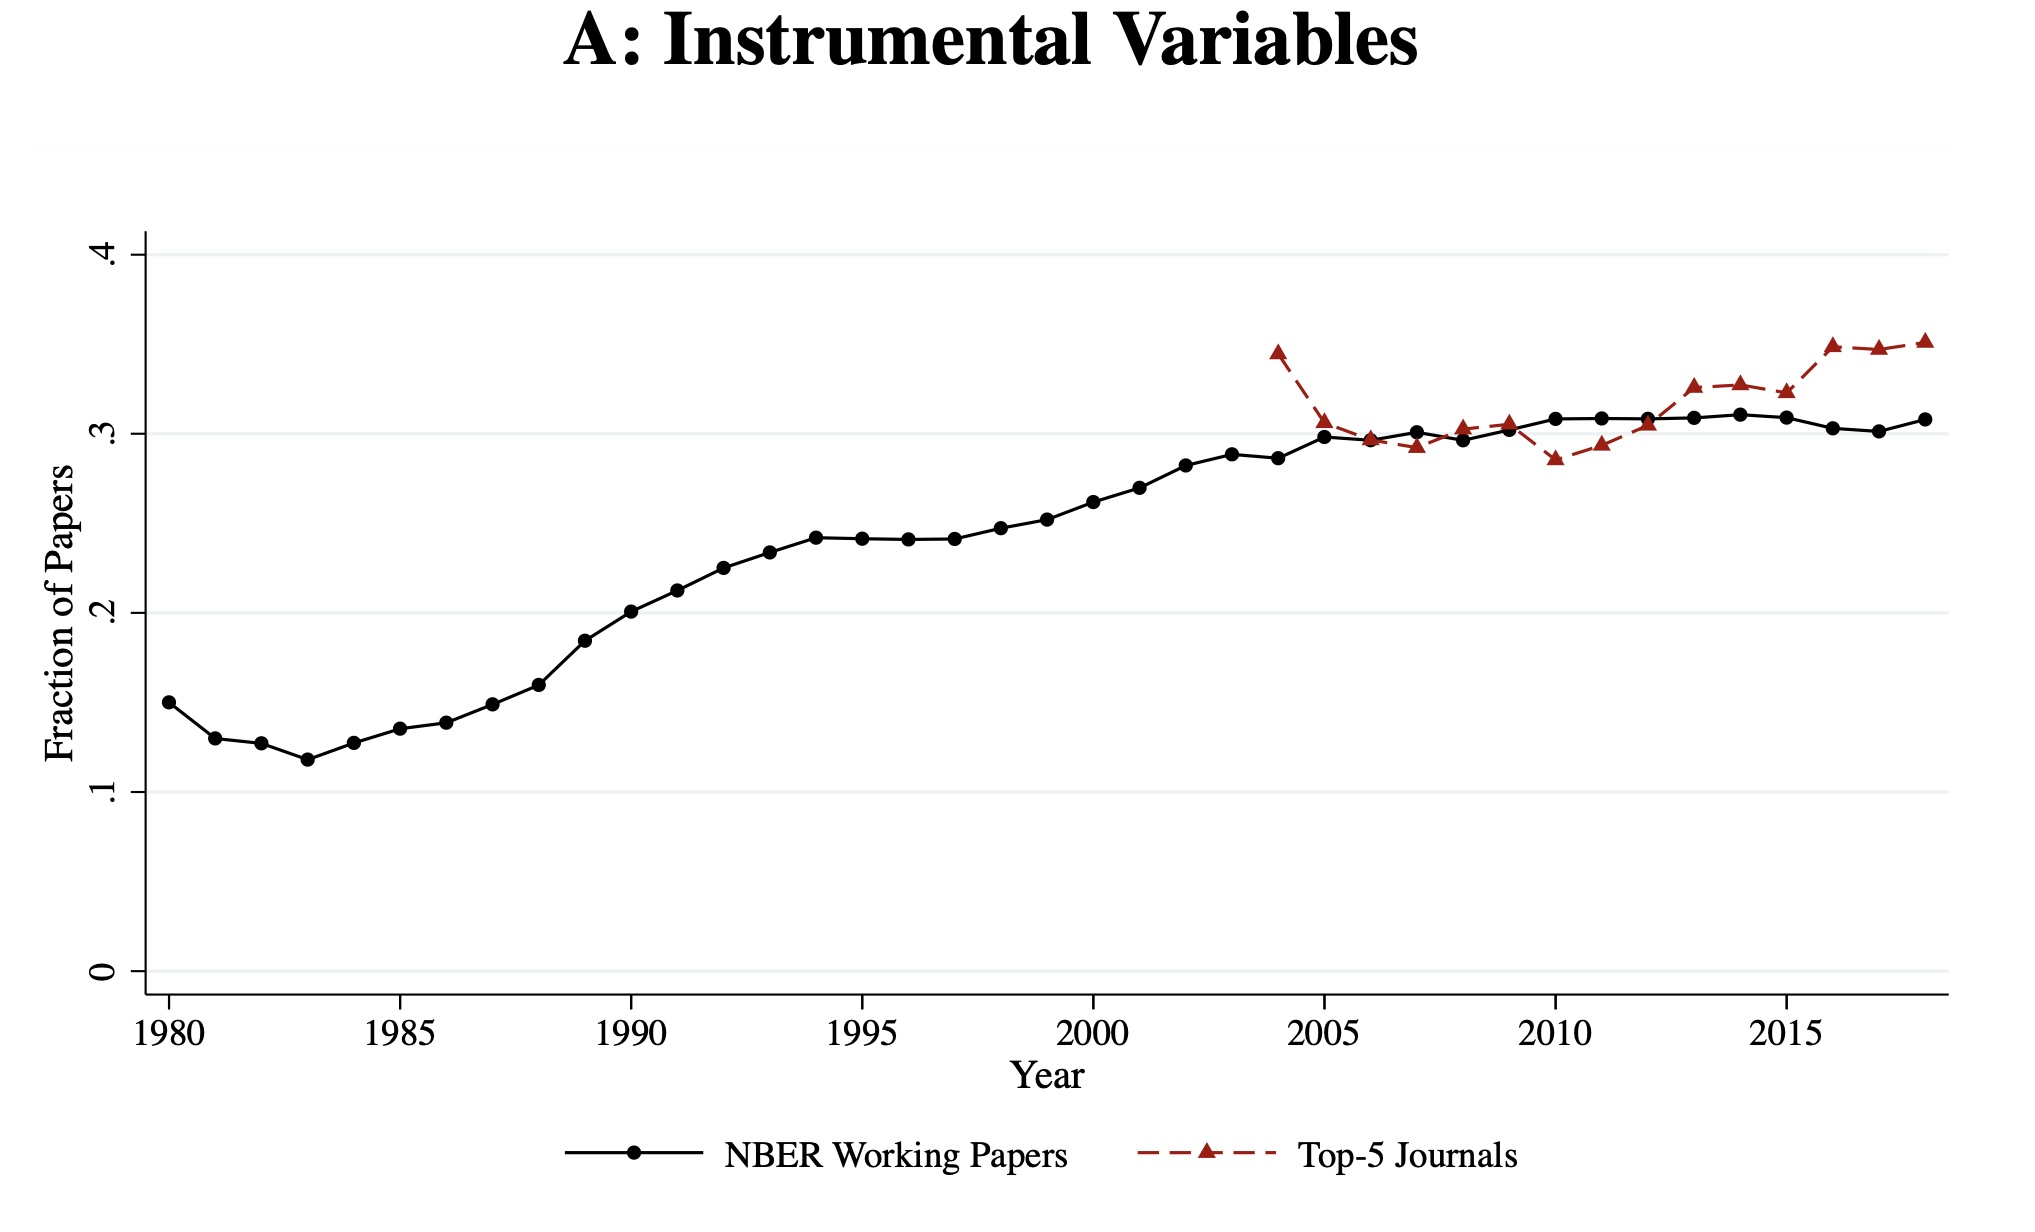
\includegraphics[scale=.15]{./lecture_includes/currie_iv}
	\end{figure}
	
\end{frame}

\begin{frame}{What is instrumental variables?}

\begin{itemize}
\item Often associated with ``natural experiments'' because an instrument is when we discovered our treatment variable randomly changed when a third seemingly inconsequential event occurred
\item Natural experiments are rarely ``good instruments'' because they often are associated with too much destruction to be useful, but the metaphor can be helpful because we often use instruments to recreate the conditions of a randomized experiment outside the lab
\item Do we find instruments or do they find us?  They tend to become apparent to us when we understand what they are as otherwise they're chameleons blending into the background

\end{itemize}

\end{frame}



	
\begin{frame}{IV from my research}

\begin{itemize}
\item Estimated the effect of growing online sex work on street prostitution arrests using commercial broadband adoption as an instrument for online sex work (Cunningham and Kendall 2010)
\item Estimated the effect of parental meth abuse on foster care and child abuse/neglect using changes in meth prices caused by shortages of ephedrine and pseudoephedrine as an instrument for meth abuse (Cunningham and Finlay 2010)
\item Estimated the price elasticity of demand for meth using the same instrument (Cunningham and Finlay 2014)
\item Estimated the effect of being classified mentally ill in jail on suicide attempts (Seward, Cunningham, Vigliotti and Clay 2022)
\end{itemize}

\end{frame}

\begin{frame}{Uses of instrumental variables}

\begin{itemize}
\item When you have unobserved confounders, IV may work
\item When you have reverse causality, IV could help
\item When you have variables being determined simultaneously (like in markets with supply and demand), then IV can step in
\item When you run an experiment (RCT, AB tests, etc.) but not everyone obeys their treatment assignment, IV will help you
\item When your treatment variable is measured with error, IV can help
\end{itemize}

\end{frame}

\begin{frame}{My Teaching Style}

\begin{enumerate}
\item Intuition first -- what is an instrument and what do you do with it?
\item Estimation second -- what are most common methods employed?
\item Interpretation -- constant treatment effects versus heterogeneous treatment effects and the LATE parameter
\item Applications -- price elasticity of demand, leniency
\end{enumerate}

\end{frame}

\begin{frame}{Constant versus heterogenous treatment effects}

Angrist and Imbens won the Nobel Prize (with Card) in October 2021 for their work on instrumental variables which focused on interpretation when treatment effects differed across a population

\begin{itemize}
\item \textbf{Constant treatment effects}: you and I both benefit the same from a college degree
\item \textbf{Heterogenous treatment effects}: college degree \emph{causes} my wages to rise by 5\% but caused yours to rise by 18\%
\end{itemize}

\bigskip

We'll start with the first but then move into the second.

\end{frame}


\begin{frame}{Instruments aren't labeled}

	\begin{itemize}
	\item Your data isn't going to come with a codebook saying ``instrumental variable''.  So how do you find it?
	\item Well, sometimes the researcher just \emph{knows}
	\item You know instruments when you see them because you know what their general structure is, and then notice them in the events and surroundings of the thing you're studying (Angrist and Krueger 2001).  
	\end{itemize}
\end{frame}


\begin{frame}{Picking a good instrument}

	\begin{itemize}
	\item Typically instruments are random events that are captured with a covariate that are highly predictive of your treatment variable but are in no other way related to the outcome
	\item If you want to use IV, then ask yourself this questions: 
		\begin{quote}
		Is there \emph{any} part of your treatment variable that is blown by the wind (i.e., random)? If so, is there a variable you know of that is associated with that randomness?
		\end{quote}
		\item In other words, is there any element in the treatment that could be construed as driven by a non-confounder (i.e., random)?  
	\end{itemize}
\end{frame}



\begin{frame}{Strangeness Example}

		\begin{itemize}
		\item What if I told you if the first two children born were of the same sex, then the mother is less likely to work.
		\item What does sex composition of first two born have to do with a mother's willingness or ability to work? \pause
		\item Unclear to an intelligent layperson why it should matter \pause which is why it is a good instrument potentially
		\end{itemize}

\end{frame}


\begin{frame}{Angrist and Evans cont.}

\begin{itemize}

		\item Many parents have both a ``stopping rule'' and a preference for having at least one child of each sex
			\begin{itemize}	
			\item If a couple whose first two kids were both boys, they will often have a third, hoping to have a girl
			\item If a couple whose first two kids were both girls, they will often have a third, hoping to have a boy
			\item But if it was boy/girl or girl/boy, they will often \textbf{stop}
			\end{itemize}
		\item Sex of your kids is essentially as good as random (around 0.51 historically chance of a boy)
		\item Josh Angrist and Bill Evans used sex ratio of first two kids as an instrument for family size to estimate effect of family size on whether a woman worked
		\end{itemize}

\end{frame}



\begin{frame}{Good instruments must be a bit strange}

\begin{itemize}
		\item On its face, it's puzzling that the first two kids' gender predicts labor market participation
		\item Instrumental variables strategies formalize this \emph{strangeness}, 
		\item Strangeness principle is the inference drawn by an intelligent layperson with no particular knowledge of the phenomena or background in statistics.
		\item Without understanding the research question (family size $\rightarrow$ maternal work), the instrument's correlation with the outcome (sex ratio of first two kids predicting maternal work) makes no sense
\end{itemize}

\end{frame}


\begin{frame}{Sunday Candy is a good instrument}

\begin{itemize}
		\item Let's listen to a few lines from ``Ultralight Beam'' by Kanye West (skip to 2:30, but then it's around 3:15)
		\item Chance the Rapper sings the following two lines

\bigskip

\begin{quote}
``I made Sunday Candy, I'm never going to hell \\


I met Kanye West, I'm never going to fail.'' \\


- Chance the Rapper
\end{quote}

	\item What does a song have to do with hell, or meeting Kanye to do with success?  
	\item These are instruments, but for what and are they good ones?
	\end{itemize}
\end{frame}

\begin{frame}{What are we missing?}

			\begin{quote}
			``I made Sunday Candy, \\
			I'm never going to hell'', 
			\end{quote}
		\begin{itemize}
		\item There must be more to this story, right?
		\item So what if it's something like this
		\end{itemize}
			\begin{quote}
			``I made Sunday Candy \\
			 \textcolor{blue}{a pastor invited me to church on Sunday}, \\
			  I'm never going to hell''
			\end{quote}

\end{frame}




\begin{frame}{Sunday Candy DAG}
	
	
	\begin{center}
	\begin{minipage}{.5\textwidth}
	
	\begin{center}
	
	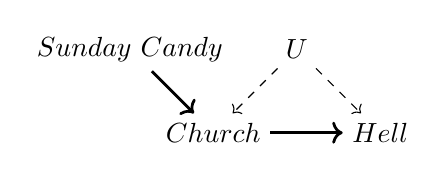
\begin{tikzpicture}[node distance=1.5cm]
	
		% nodes - for left-hand DAG %
		\node[text centered] (u) {$U$};
		\node[below right of  = u, text centered] (y) {$Hell$};
		\node[below left of = u, text centered] (d) {$Church$};
		\node[above left of = d, text centered] (z) {$Sunday\ Candy$};
 
		% edges %
		\draw[->, line width=1] (d) -- (y);
		\draw[->, line width=1] (z) -- (d);
		\draw[dashed, ->] (u) -- (y);
		\draw[dashed, ->] (u) -- (d);

		\end{tikzpicture}
		\end{center}
		\end{minipage}


	\end{center}


\end{frame}	


\begin{frame}{Kanye West is a bad instrument}

\begin{itemize}
\item Chance long idolized and was inspired by Kanye West -- both Chicago, both very creative hip hop artists
\item Kanye West is not a good instrument for Chance's inspiration, though, because Kanye West can singlehandedly make a person's career
\item Kanye is not strange enough
\end{itemize}

\end{frame}


\begin{frame}{Kanye West DAG}
	
	
	\begin{center}
	\begin{minipage}{.5\textwidth}
	
	\begin{center}
	
	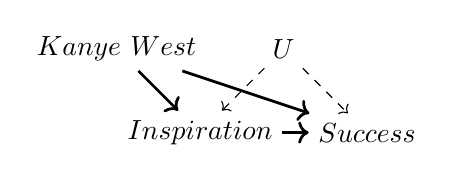
\begin{tikzpicture}[node distance=1.5cm]
	
		% nodes - for left-hand DAG %
		\node[text centered] (u) {$U$};
		\node[below right of  = u, text centered] (y) {$Success$};
		\node[below left of = u, text centered] (d) {$Inspiration$};
		\node[above left of = d, text centered] (z) {$Kanye\ West$};
 
		% edges %
		\draw[->, line width=1] (d) -- (y);
		\draw[->, line width=1] (z) -- (d);
		\draw[->, line width=1] (z) -- (y);
		\draw[dashed, ->] (u) -- (y);
		\draw[dashed, ->] (u) -- (d);

		\end{tikzpicture}
		\end{center}
		\end{minipage}


	\end{center}


\end{frame}	


\begin{frame}{Some questions you need to be asking}

\begin{enumerate}
	\item Is our instrument highly correlated with the treatment? With the outcome? Can we see evidence for this?
	\item Are there random reasons why our treatment changes? Why do you think that?
	\item Is the instrument independent of confounders?  Why do you think that?
	\item Could the instrument affect outcomes directly? Why do you think that?
\end{enumerate}

\end{frame}




\section{Estimators}

\subsection{Two Step}

\begin{frame}{Two step vs Minimum Distance}

\begin{itemize}
\item The two-stage least squares (2SLS) estimator was developed by Theil (1953) and Basman (1957) independently
\item Kolesa\'r has a helpful distinction: two step (Wald, 2 Sample IV, JIVE, UJIVE, 2SLS) vs minimum distance estimators (LIML)
\item Too much to review as IV is a \emph{huge} area, so I will focus on a few things, starting with two stage least squares (2SLS)
\item 2SLS is basically the workhorse IV model, though it can have some issues because of its finite sample bias with weak instruments
\end{itemize}

\end{frame}




\begin{frame}{Wald estimator}

\begin{eqnarray*}
Y = \alpha + \delta S + \gamma A + \nu
\end{eqnarray*}
where $Y$ is log earnings, $S$ is years of schooling, $A$ is unobserved ability, and $\nu$ is the error term

\begin{itemize}
	\item Suppose there exists a variable, $Z_i$, that is correlated with $S_i$ .
	\item We can estimate $\delta$ with this variable, $Z$:
\end{itemize}

\end{frame}


\begin{frame}{Deriving Wald}
	
		\begin{eqnarray*}
		Cov(Y,Z) 	&=& Cov(\alpha + \delta{S} + \gamma{A} + \nu, Z) \\
				&=&	E[(\alpha + \delta{S} + \gamma{A} + \nu)  Z] - E[\alpha + \delta{S} + \gamma{A} + \nu]E[Z] \\
				&=& \{\alpha E(Z) - \alpha E(Z) \} + \delta \{ E(SZ) - E(S)E(Z)\} \\
				&& + \gamma \{E(AZ) - E(A)E(Z) \} + E(\nu Z) - E(\nu)E(Z) \\
		Cov(Y,Z)	&=& \delta Cov(S,Z) + \gamma Cov(A,Z) + Cov(\nu,Z)
		\end{eqnarray*}
		Divide both sides by $Cov(S,Z)$ and the first term becomes $\delta$, the LHS becomes the ratio of the reduced form to the first stage, plus two other scaled terms.
\end{frame}

\begin{frame}{Consistency}

	\begin{itemize}
	\item What conditions must hold for a valid IV design?
		\begin{itemize}
		\item  $Cov(S,Z)\neq{0}$ -- ``first stage'' exists.  $S$ and $Z$ are correlated 
		\item $Cov(A,Z)=Cov(\nu ,Z)=0$ -- ``exclusion restriction''.  This means $Z$ that orthogonal to the factors in $\nu$, such as unobserved ability, A, as well as the structural disturbance term, $\nu$
		\end{itemize}
	\item Combine $A$ and $\nu$ into a composite error term $\eta$ for simplicity
	\item Assuming the first stage exists and that the exclusion restriction holds, then we can estimate $\delta$ with $\delta_{Wald}$:
	\end{itemize}
	\begin{eqnarray*}
	\text{plim }\widehat{\delta}_{Wald}&=& \delta + \gamma \frac{Cov(\eta,Z)}{Cov(S,Z)} \\
	&=&\delta
	\end{eqnarray*}
\end{frame}









\begin{frame}{Two Sample IV}

	\begin{itemize}
	\item Wald can be implemented in exotic ways, even across datasets
		\begin{enumerate}
		\item Dataset 1 needs information on the outcome and the instrument -- Cov(Y,Z)
		\item Dataset 2 needs  information on the treatment and the instrument -- Cov(D,Z)
		\end{enumerate}
	\item This is known as ``Two sample IV'' because there are two \emph{samples} involved, rather than the traditional one sample.
	\item Once we define what IV is measuring carefully, you will see why this works.
	\end{itemize}
\end{frame}


\begin{frame}{Two-stage least squares concepts}
	
	\begin{itemize}
	\item Causal model.  Your main research question:$$Y_i=\alpha + \delta{S_i} + \eta_i$$
	\item First-stage regression. Gets the name because of two-stage least squares:$$S_i = \gamma + \rho{Z_i} + \zeta_i$$
	\item Second-stage regression. Notice the fitted values, $\widehat{S}$:$$Y_i=\beta + \delta{\widehat{S_i}}+\nu_i$$
	\item Reduced form regression: $Y$ regressed onto the instrument:$$Y_i=\psi + \pi{Z_i} + \varepsilon_i$$
	\end{itemize}
\end{frame}








\begin{frame}{Two-stage least squares language}

Suppose you have a sample of data on $Y$, $S$, and $Z$. For each observation $i$ we assume the data are generated according to
		\begin{eqnarray*}
		Y_i &=& \alpha + \delta{S}_i + \eta_i \text{ (causal model)}\\
		S_i &=& \gamma + \rho{Z}_i + \zeta_i \text{ (first stage)} 
		\end{eqnarray*}where $Cov(Z,\eta_i)=0$ (strangeness, hereafter exclusion) and $\rho\neq{0}$ (relevance, hereafter non-zero first stage)

\end{frame}

\begin{frame}{Two-stage least squares language}

		\begin{eqnarray*}
		Y_i&=&\psi + \pi{Z_i} + \varepsilon_i \text{ (reduced form)} \\
		S_i &=& \gamma + \rho{Z}_i + \zeta_i \text{ (first stage)} 
		\end{eqnarray*}
		
		\bigskip
		
We can calculate the ratio of ``reduced form'' ($\pi$) to ``first stage'' coefficient ($\rho$) using the Wald IV estimator:
		\begin{eqnarray*}
		\widehat{\delta}_{Wald} = \frac{ Cov(Z,Y)} {Cov(Z,S)} = \frac{ \frac{Cov(Z,Y)}{Var(Z)}}{ \frac{Cov(Z,S)}{Var(Z)}} = \frac{\widehat{\pi}}{\widehat{\rho}}
		\end{eqnarray*}

\end{frame}



\begin{frame}{Two-stage least squares}

Carry over from previous slide

\bigskip

		\begin{eqnarray*}
		\widehat{\delta}_{Wald} = \frac{ Cov(Z,Y)} {Cov(Z,S)} = \frac{ \frac{Cov(Z,Y)}{Var(Z)}}{ \frac{Cov(Z,S)}{Var(Z)}} = \frac{\widehat{\pi}}{\widehat{\rho}}
		\end{eqnarray*}

\bigskip

Rewrite $\widehat{\rho}$ as\begin{eqnarray*}
	\widehat{\rho} &=&  \frac{Cov(Z,S)}{Var(Z)} \\
\widehat{\rho}Var(Z)	&=& Cov(Z,S) 
	\end{eqnarray*}

\end{frame}


\begin{frame}{Two-stage least squares}

Multiply Wald IV by $\frac{\widehat{\rho}}{\widehat{\rho}}$  (also note the subscript -- we are moving now into 2SLS)

	\begin{eqnarray*}
	\widehat{\delta}_{2sls} &=& \frac{ Cov(Z,Y)}{ Cov(Z,S)} = \frac{\widehat{\rho}Cov(Z,Y)}{\widehat{\rho}Cov(Z,S)} \\
	\end{eqnarray*}

Substitute $Cov(Z,S) = \widehat{\rho}Var(Z) $ and simplify as constants disappear in covariance and variance

	\begin{eqnarray*}
	\widehat{\delta}_{2sls} &=& \frac{\widehat{\rho}Cov(Z,Y)}{\widehat{\rho}Cov(Z,S)} = \frac{\widehat{\rho}Cov(Z,Y)}{\widehat{\rho}^2Var(Z)}  \\
	&=&\frac{Cov(\widehat{\rho}Z,Y)}{Var(\widehat{\rho}Z)} 
	\end{eqnarray*}

\end{frame}

\begin{frame}{Two-stage least squares}
	
Recall $$ S_i = \gamma + \rho{Z}_i + \zeta_i \text{ (first stage)} $$So after estimation, we get $$\widehat{S}=\widehat{\gamma} + \widehat{\rho}Z \text{ (fitted values)}$$  
Substitute for $\widehat{S}$ for $\widehat{\rho}Z$ ($\widehat{\gamma}$ drops out)
		\begin{eqnarray*}
		\widehat{\delta}_{2sls} &=& \frac{Cov(\widehat{\rho}Z,Y)}{Var(\widehat{\rho}Z)} =  \frac{Cov(\widehat{S},Y)}{Var(\widehat{S})}
		\end{eqnarray*}
		
		

\end{frame}

\begin{frame}[plain]

		\begin{proof}
		We will show that $\widehat{\delta}Cov(Y,Z) = Cov(\widehat{S},Y)$.  I will leave it to you to show that $Var(\widehat{\delta}Z) = Var(\widehat{S})$
		\begin{eqnarray*}
		Cov(\widehat{S},Y) &=& E[\widehat{S}Y] - E[\widehat{S}]E[Y] \\
		&=& E(Y[\widehat{\rho} + \widehat{\delta}Z]) - E(Y)E(\widehat{\rho} + \widehat{\delta}Z) \\
		&=& \widehat{\rho}E(Y) + \widehat{\delta}E(YZ) - \widehat{\rho}E(Y) - \widehat{\delta}E(Y)E(Z) \\
		&=&\widehat{\delta}[E(YZ) - E(Y)E(Z)] \\
		Cov(\widehat{S},Y) &=& \widehat{\delta}Cov(Y,Z)
		\end{eqnarray*}
		\qedhere
		\end{proof}

\end{frame}


\begin{frame}{Intuition of 2SLS}
	
	\begin{itemize}
	\item Intuition is that 2SLS replaces $S$ with the fitted values $\widehat{S}$ from the first stage regression of $S$ onto $Z$ and all other covariates 
	\item Our previous slides showed that 2SLS and the ratio of reduced form and first stage were equivalent though
	\item By using the fitted values of the endogenous regressor from the first stage regression, our regression now uses \emph{only} the quasi-random variation in the treatment due to the instrumental variable itself (only the random parts of schooling remain)
	\end{itemize}
\end{frame}








\begin{frame}{Finite sample problems with 2SLS}

Suppose you have a sample of data on $Y$, $X$, and $Z$. For each observation $i$ we assume the data are generated according to
		\begin{eqnarray*}
		Y_i &=& \alpha + \delta{S}_i + \eta_i \\
		S_i &=& \gamma + \rho{Z}_i + \zeta_i
		\end{eqnarray*}where $Cov(Z,\eta_i)=0$ and $\rho\neq{0}$.

\end{frame}


\begin{frame}{Finite sample problems with 2SLS}

Plug in covariance and write out the following:
		\begin{eqnarray*}
		\widehat{\delta_{2sls}} &=& \frac{Cov(Z,Y)}{Cov(Z,S)} \\
		&=& \frac{ \frac{1}{n}\sum_{i=1}^n(Z_i - \overline{Z})(Y_i - \overline{Y})}{\frac{1}{n}\sum_{i=1}^n(Z_i - \overline{Z})(S_i - \overline{S})} \\
		&=& \frac{ \frac{1}{n} \sum_{i=1}^n(Z_i - \overline{Z})Y_i}{ \frac{1}{n} \sum_{i=1}^n (Z_i-\overline{Z})S_i}
		\end{eqnarray*}

\end{frame}

\begin{frame}{Finite sample problems with 2SLS}

Substitute the causal model definition of $Y$ to get:
		\begin{eqnarray*}
		\widehat{\delta_{2sls} }&=& \frac{ \frac{1}{n} \sum_{i=1}^n (Z_i -\overline{Z})\{ \alpha + \delta{S}_i + \eta_i \}}{\frac{1}{n} \sum_{i=1}^n (Z_i - \overline{Z})S_i} \\
		&=& \delta + \frac{\frac{1}{n} (Z_i - \overline{Z})\eta_i}{\frac{1}{n}\sum_{i=1}^n(Z_i - \overline{Z})S_i} \\
		&=& \delta + \text{"small if \emph{n} is large"}
		\end{eqnarray*}Where did the first term go? Why did the second term become $\delta$? Why might the second term not be zero even under exclusion?

\end{frame}	


\begin{frame}{Intuition of 2SLS}
	
	\begin{itemize}
	\item Two stage least squares is nice because in addition to being an estimator, there's also great intuition contained in it which you can use as a device for thinking about IV more generally. 
	\item The intuition is that 2SLS estimator replaces $S$ with the fitted values of $S$ (i.e., $\widehat{S}$) from the first stage regression of $S$ onto $Z$ and all other covariates.  
	\item By using the fitted values of the endogenous regressor from the first stage regression, our regression now uses \emph{only} the exogenous variation in the regressor due to the instrumental variable itself
	\end{itemize}
\end{frame}

\begin{frame}{Intuition of IV in 2SLS}

\begin{itemize}
	\item \dots but think about it -- that variation was there before, but was just a subset of all the variation in the regressor
	\item Go back to what we said in the beginning - we need the endogenous variable to have pieces that are random, and IV finds them.
	\item Instrumental variables therefore reduces the variation in the data, but that variation which is left is 
\emph{exogenous}
\end{itemize}

\end{frame}
	



\begin{frame}{Software}



Probably not a bad idea to estimate both reduced form and first stage, just to check everything is sensible, but ultimately you want to use software because second stage standard errors are wrong

\bigskip

\begin{itemize}
	\item Estimate this in Stata using -ivregress 2sls-.
	\item Estimate this in R -ivreg()- which is in the AER package
	\item Lots of options, like -linearmodels-, in python

\end{itemize}

\end{frame}



\subsection{Weak instruments}

\begin{frame}{Weak instruments}

\begin{quote}
``In instrumental variables regression, the instruments are called weak if their correlation with the endogenous regressors, conditional on any controls, is close to zero.'' -- Andrews, Stock and Sun (2018)
\end{quote}

\end{frame}

\begin{frame}{Weak instruments}

\begin{itemize}
\item Weak instruments can happen if the two variables are independent or the sample is small
\item If you have a weak instrument, then the bias of 2SLS is centered on the bias of OLS and the cure ends up being worse than the disease
\item This brought into sharp focus with Angrist and Krueger (1991) quarter of birth study and some papers that followed
\end{itemize}

\end{frame}

\begin{frame}{My March 2022 Interview with Angrist}

Before we dive into the paper, though, let's listen to Angrist discuss the history

\bigskip

\url{https://youtu.be/ApNtXe-JDfA?t=2348}

\bigskip

Somewhat inspiring to hear how Angrist reframed the weak instrument problem which his paper with Krueger brought into crisp focus

\end{frame}


\begin{frame}{Angrist and Krueger (1991)}
	
	\begin{itemize}
	\item In practice, it is often difficult to find convincing instruments -- usually because potential instruments don't satisfy the exclusion restriction
	\item But in an early paper in the causal inference movement, Angrist and Krueger (1991) wrote a very interesting and influential study instrumental variable 
	\item They were interested in schooling's effect on earnings and instrumented for it with \emph{which quarter of the year you were born}
	\item Remember Chance quote - what the heck would birth quarter have to do with earnings such that it was an excludable instrument?
	\end{itemize}
	
\end{frame}


\begin{frame}{Compulsory schooling}

\begin{itemize}

	\item In the US, you could drop out of school once you turned 16
	\item ``School districts typically require a student to have turned age six by January 1 of the year in which he or she enters school'' (Angrist and Krueger 1991, p. 980)
	\item Children have different ages when they start school, though, and this creates different lengths of schooling at the time they turn 16 (potential drop out age):
	\end{itemize}
	
\end{frame}

\begin{frame}[plain]
\begin{figure}[htb]
\centering
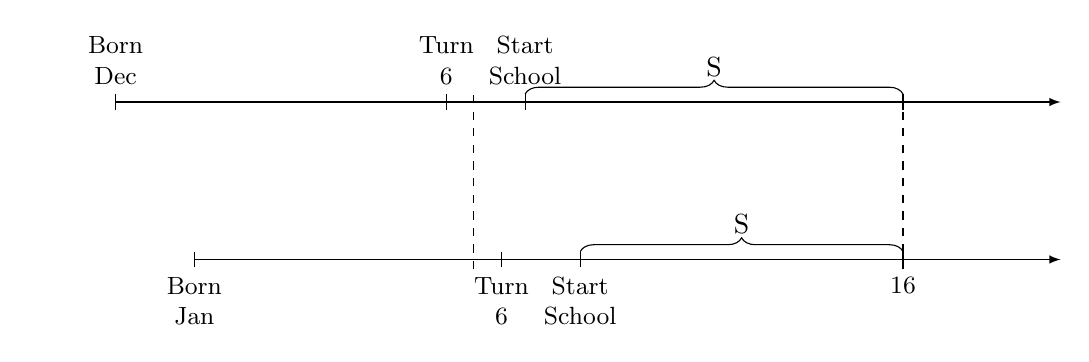
\begin{tikzpicture}
	\draw [-{latex}] (0,2) -- (12,2);
	\draw [-{latex}] (1,0) -- (12,0);
	
	\draw (0,1.9) -- (0,2.1) node [anchor=south, pos=1, text width=2cm, align=center, font=\small] {Born\\ Dec};
	\draw (4.2,1.9) -- (4.2,2.1) node [anchor=south, pos=1, text width=2cm, align=center, font=\small] {Turn\\ 6};
	\draw (5.2,1.9) -- (5.2,2.1) node [anchor=south, pos=1, text width=2cm, align=center, font=\small] {Start\\ School};
	\draw (10,1.9) -- (10,2.1);
	
	\draw (1,-0.1) -- (1,0.1) node [anchor=north, pos=0, text width=2cm, align=center, font=\small] {Born\\ Jan};
	\draw (4.9,-0.1) -- (4.9,0.1) node [anchor=north, pos=0, text width=2cm, align=center, font=\small] {Turn\\ 6};
	\draw (5.9,-0.1) -- (5.9,0.1) node [anchor=north, pos=0, text width=2cm, align=center, font=\small] {Start\\ School};
	\draw (10,-0.1) -- (10,0.1) node [anchor=north, pos=0, text width=2cm, align=center, font=\small] {16};
	
	\draw [dashed] (4.55,-0.125) -- (4.55,2.125);
	\draw [dashed] (10,-0.125) -- (10,2.125);
	
	\draw [decorate, decoration={brace, amplitude=5pt, raise=0pt}] (5.2,2.1) -- (10,2.1) node [pos=0.5,anchor=south, yshift=0.1cm] {S};
	\draw [decorate, decoration={brace, amplitude=5pt, raise=0pt}] (5.9,0.1) -- (10,0.1) node [pos=0.5,anchor=south, yshift=0.1cm] {S};
		
\end{tikzpicture}

\end{figure}
If you're born in the fourth quarter, you hit 16 with more schooling than those born in the first quarter
\end{frame}

\begin{frame}{Visuals}

\begin{itemize}
\item You need good data visualization for IV partly because of the scrutiny around the design
\item The two pieces you should be ready to build pictures for are the first stage and the reduced form
\item Angrist and Krueger (1991) provide simple, classic and compelling pictures of both
\end{itemize}

\end{frame}



\begin{frame}{First Stage}
	
	 Men born earlier in the year have lower schooling. This indicates that there is a first stage. Notice all the 3s and 4s at the top. But then notice how it attenuates over time \dots
	
	\begin{figure}
	\includegraphics{./lecture_includes/qob_2.pdf}
	\end{figure}
	
\end{frame}


\begin{frame}{Reduced Form}
	
	 Do differences in schooling due to different quarter of birth translate into different earnings?
	
	\begin{figure}
	\includegraphics{./lecture_includes/qob_3.pdf}
	\end{figure}
	
\end{frame}

\begin{frame}{Two Stage Least Squares model}
	
	\begin{itemize}
	\item The causal model is $$Y_i = X \pi + \delta S_i + \varepsilon$$
	\item The first stage regression is:$$S_i=X\pi_{10} + \pi_{11}Z_i + \eta_{1i}$$
	\item The reduced form regression is:$$Y_i=X\pi_{20} + \pi_{21}Z_i+\eta_{2i}$$
	\item The covariate adjusted IV estimator is the sample analog of the ratio, $\frac{\pi_{21}}{\pi_{11}}$
	\end{itemize}

\end{frame}

\begin{frame}{Two Stage Least Squares}
	
	\begin{itemize}
	\item Angrist and Krueger instrument for schooling using three quarter of birth dummies:  a dummies for 1st, 2nd and 3rd qob
	\item Their estimated first-stage regression is:$$S_i=X\pi_{10} + Z_{1i}\pi_{11} + Z_{2i}\pi_{12} + Z_{3i}\pi_{13}+\eta_1$$
	\item The second stage is the same as before, but the fitted values are from the new first stage
	\end{itemize}

\end{frame}


\begin{frame}{First stage regression results}

	 Quarter of birth is a strong predictor of total years of education
	
	\begin{figure}
	\includegraphics{./lecture_includes/qob_5.pdf}
	\end{figure}

\end{frame}




\begin{frame}{IV Estimates Birth Cohorts 20-29, 1980 Census}
	
	\begin{figure}
	\includegraphics{./lecture_includes/qob_7.pdf}
	\end{figure}
	
\end{frame}




\begin{frame}{More instruments}

	\begin{figure}
	\includegraphics[scale=.25]{./lecture_includes/weak_qob1.png}
	\end{figure}
	

\end{frame}


\begin{frame}{Problem enters with many quarter of birth interactions}
	
	\begin{itemize}
	\item They want to increase the precision of their 2SLS estimates, so they load up their first stage with more instruments
	\item Specifications with 30 (quarter of birth $\times$ year) dummy variables and 150 (quarter of birth $\times$ state) instruments
		\begin{itemize}
		\item What's the intuition here?  The effect of quarter of birth may vary by birth year or by state
		\item By interacting their instrument with variables, they are ``saturating'' their 2SLS regression model (more on that later)
		\end{itemize}
	\item It reduced the standard errors, but that comes at a cost of potentially having a weak instruments problem
	\end{itemize}
	
\end{frame}




\begin{frame}{More instruments}

	\begin{figure}
	\includegraphics[scale=.25]{./lecture_includes/weak_qob2.png}
	\end{figure}
	

\end{frame}


\begin{frame}{More instruments}

	\begin{figure}
	\includegraphics[scale=.18]{./lecture_includes/weak_qob3.png}
	\end{figure}
	

\end{frame}


\begin{frame}{Weak Instruments}
	
	\begin{itemize}
	\item Important paper suggesting OLS and 2SLS were pretty similar, as well as the power of natural experiments (``plausibly exogenous'')
	\item But in the early 1990s, a number of papers highlighted that IV can be \emph{severely} biased -- in particular, when instruments have only a weak correlation with the endogenous variable of interest and when many instruments are used to instrument for one endogenous variable (i.e., there are many overidentifying restrictions).
	\item In the worst case, if the instruments are so weak that there is no first stage, then the 2SLS sampling distribution is centered on the probability limit of OLS
	\end{itemize}
\end{frame}



\begin{frame}{Matrices and instruments}

\begin{itemize}
	\item The causal model of interest is: $$Y=\beta X + \nu$$
	\item Matrix of instrumental variables is Z with the first stage equation:$$X = {Z'}\pi + \eta$$
\end{itemize}

\end{frame}

\begin{frame}{Weak instruments and bias towards OLS}

\begin{itemize}
	\item If $\nu_i$ and $\eta_i$ are correlated, estimating the first equation by OLS would lead to biased results, wherein the OLS bias is:$$E[\beta_{OLS} - \beta] = \frac{ Cov(\nu, X)}{Var(X)}$$
	\item If $\nu_i$ and $\eta_i$ are correlated the OLS bias is therefore: $\frac{\sigma_{\nu \eta}}{\sigma^2_\eta}$
\end{itemize}

\end{frame}


\begin{frame}{Weak instruments and 2SLS bias towards OLS}
	
	\begin{itemize}
	\item We can derive the approximate bias of 2SLS as:$$E[\widehat{\beta}_{2SLS} - \beta] \approx \frac{\sigma_{\nu \eta}}{\sigma^2_\eta} \frac{1}{F+1}$$
	\item Consider the intuition all that work bought us now: if the first stage is weak (i.e, $F\rightarrow{0}$), then the bias of 2SLS approaches $\frac{\sigma_{\nu \eta}}{\sigma^2_\eta}$
	\end{itemize}
\end{frame}

\begin{frame}{Weak instruments and bias towards OLS}

\begin{itemize}
	\item This is the same as the OLS bias as for $\pi=0$ in the second equation on the earlier slide (i.e., there is no first stage relationship) $\sigma^2_x = \sigma^2_\eta$ and therefore the OLS bias $\frac{\sigma_{\nu \eta}}{\sigma^2_\eta}$ becomes $\frac{\sigma_{\nu \eta}}{\sigma^2_\eta}$.
	\item But if the first stage is very strong ($F\rightarrow{\infty}$) then the 2SLS bias is approaching 0.
	\item Cool thing is -- you can test this with an F test on the joint significance of $Z$ in the first stage
	\item It's absolutely critical therefore that you choose instruments that are strongly correlated with the endogenous regressor, otherwise the cure is worse than the disease
\end{itemize}

\end{frame}

\begin{frame}{Weak Instruments - Adding More Instruments}
	
	\begin{itemize}
	\item Adding more weak instruments will increase the bias of 2SLS
		\begin{itemize}
		\item By adding further instruments without predictive power, the first stage $F$-statistic goes toward zero and the bias increases
		\item We will see this more closely when we cover the leniency design
		\end{itemize}
	\item If the model is ``just identified'' -- mean the same number of instrumental variables as there are endogenous covariates -- weak instrument bias is less of a problem
	\end{itemize}
\end{frame}

\begin{frame}{Weak instrument problem}

\begin{itemize}
	\item After Angrist and Krueger study, there were new papers highlighting issues related to weak instruments and finite sample bias
	\item Key papers are Nelson and Startz (1990), Buse (1992), Bekker (1994) and especially Bound, Jaeger and Baker (1995)
	\item Bound, Jaeger and Baker (1995) highlighted this problem for the Angrist and Krueger study.  
\end{itemize}

\end{frame}

\begin{frame}{Bound, Jaeger and Baker (1995)}

Remember, AK present findings from expanding their instruments to include many interactions (i.e., saturated model)
		\begin{enumerate}
		\item Quarter of birth dummies $\rightarrow$ 3 instruments
		\item Quarter of birth dummies $+$ (quarter of birth) $\times$ (year of birth) $+$ (quarter of birth) $\times$ (state of birth) $\rightarrow$ 180 instruments
		\end{enumerate}
So if any of these are weak, then the approximate bias of 2SLS gets worse

\end{frame}


\begin{frame}{Adding instruments in Angrist and Krueger}
	
	\begin{figure}
	\includegraphics{./lecture_includes/ak_iv1.pdf}
	\end{figure}
	
Adding more weak instruments reduced the first stage $F$-statistic and increases the bias of 2SLS. Notice its also moved closer to OLS. 
	
\end{frame}

\begin{frame}{Adding instruments in Angrist and Krueger}
	
	\begin{figure}
	\includegraphics{./lecture_includes/ak_iv2.pdf}
	\end{figure}
	
More instruments increase precision, but drive down $F$, therefore we know the problem has gotten worse
	
\end{frame}




\begin{frame}{IV advice: Weak instruments}

	\begin{itemize}
	\item Excellent review by Keane and Neal (2021) ``A Practical Guide to Weak Instruments''  as well as Andrews, Stock and Sun (2018)
	\item Stock, Wright and Yogo (2002) found that $F$ statistics on the excludability of the instrument from the first stage greater than 10 performed well in Monte Carlos with homoskedasticity, but 2SLS is has poor properties here
		\begin{itemize}
		\item Under powered
		\item Artificially low standard errors when endogeneity is severe
		\item This causes $t$-tests to be misleading
		\end{itemize}
	\end{itemize}

\end{frame}

\begin{frame}{IV advice: Weak instruments}

\begin{quote}
``In the leading case with a single endogenous regressor, we recommend that researchers judge instrument strength based on the effective F-statistic of Montiel Olea and Pflueger (2013).  If there is a single instrument, we recommend reporting identification robust Anderson-Rubin confidence intervals. These are effective regardless of the strength of the instruments, and so should be reported regardless of the value of the first stage F.  Finally, if there are multiple instruments, the literature has not yet converged on a single procedure, but we recommend choosing from among the several available robust procedures that are efficient when the instruments are strong.'' -- Andrews, Stock and Sun (2018)
\end{quote}

\end{frame}


\begin{frame}{IV advice: Weak instruments}

\begin{itemize}
	\item Anderson-Rubin greatly alleviate this problem and should be used even with very strong instruments provided the first-stage $F$ is well above 10 (Lee, et al. 2020 say 104.7)
	\item Higher thresholds are recommended, and even then robust tests are suggested unless $F$ is in the thousands
	\item Keane and Neal (2021) write, ``to avoid over-rejecting the null when $\beta_{2SLS}$ is shifted in the direction of the OLS bias, one should rely on the Anderson-Rubin test rather than the $t$-test even when the first-stage $F$-statistic is in the thousands.'' 
\end{itemize}

\end{frame}

\begin{frame}{Heteroskedastic DGP}

\begin{itemize}
\item Assessing acceptable first stage $F$ statistics means in practice considering the impact of heteroskedasticity
\item With multiple instruments, it is inappropriate to use either a conventional or heteroskedasticity robust $F$-tsest to gauge instrument strength
\item Andrews, et al. (2019) suggest the Olea and Pflueger (2013) effective first-stage $F$ statistic
\item Single instrument just-identified case reduces to the conventional robust $F$ and the Kleibergen and Paap (2006) Wald
\end{itemize}

\end{frame}







\subsection{Local average treatment effects}

\begin{frame}{Constant vs heterogenous treatment effects}

\begin{itemize}
\item IV was modeled using realized outcomes, which clouded causal inference
\item But also tended to assume constant treatment effects
\item When you introduced heterogenous treatment effects, IV became more complex 
\end{itemize}

\end{frame}

\begin{frame}{Some background}

\begin{itemize}
\item October 2021's Nobel Prize in economics went to Card, Angrist and Imbens (the last two for work 1990s work on IV)
\item Angrist writes a dissertation using randomized instruments (Vietnam draft), goes to Harvard, overlaps with Imbens for a year, they are mentored by Gary Chamberlain, work with Don Rubin, write their famous LATE paper
\item Chamberlain recommends modifying Rubin's potential outcomes framework (instead of their original latent index modeling) and that seems to make the work more generally attractive (outside economics)
\item Let's spend twenty minutes listening to them
\end{itemize}

\end{frame}

\begin{frame}{Angrist, Imbens and Harvard}


Josh Angrist on the negative results at the time (10 min)

\url{https://youtu.be/ApNtXe-JDfA?t=1885}

Guido Imbens on the reception of their work (10 min)

\url{https://youtu.be/cm8V65AS5iU?t=799}

\end{frame}




\begin{frame}{Potential treatment concept}
	
``Potential treatment status'' ($D^j$) is like potential outcomes the thought experiment; it's not the observed treatment status $D$ until we switch between them with the instrument's assignment
\bigskip
		\begin{itemize}
		\item $D^1_{i} = i$'s treatment status when $Z_i=1$
		\item $D^0_{i} = i$'s treatment status when $Z_i=0$
		\end{itemize}
\bigskip
We'll represent outcomes as a function of both treatment status and instrument status. In other words, $Y_i(D_i=0,Z_i=1)$ is represented as $Y_i(0,1)$

\end{frame}




\begin{frame}{Identification}
		
	\begin{enumerate}
	\item Stable Unit Treatment Value Assumption (SUTVA)
	\item Random Assignment
	\item Exclusion Restriction
	\item Nonzero First Stage
	\item Monotonicity
	\end{enumerate}
\end{frame}


\begin{frame}{SUTVA}

\begin{block}{SUTVA with respect to IV}
In the IV context, SUTVA means the \textbf{potential treatments} for any unit do not (1) vary with the instruments assigned to other units, and for each unit, (2) there are no different forms of versions of each instrument level, which lead to different potential treatments
\end{block}

\bigskip

Once you make $D^1_i$, $D^0_i$ based on a scalar, you've invoked SUTVA because this means your potential outcome is not based on other's assignment and it means there's no hidden variation in the instrument

\bigskip

Example:   The instrument is a randomly generated draft number. When your friend, $i'$, gets drafted, you, $i$, somehow get drafted too even though you didn't get assigned with your draft number


\end{frame}

		


\begin{frame}{Independence assumption}
	
	\begin{block}{Independence assumption}
	$\{Y_i(D^1_i,1),Y_i(D^0_i,0),D^1_{i},D^{0}_i\} \independent{Z}_i$
	\end{block}

\begin{itemize}	
\item Instruments are assigned independent of potential treatment status and potential outcomes
\item Independence is ensured by physical randomization, but perhaps other assignments could too (e.g., alphabetized assignment)
\item Example: Random draft numbers generated by a random number generator
\end{itemize}

\end{frame}


\begin{frame}{Independence}

		 \textbf{Implications of independence}: First stage measures the causal effect of $Z_i$ on $D_i$:
			\begin{eqnarray*}
			E[D_i|Z_i=1] - E[D_i|Z_i=0] &=& E[D^1_{i} | Z_i = 1] - E[D^0_{i}|Z_i = 0] \\
			&=& E[D^1_{i} - D^0_{i}]
			\end{eqnarray*}

\end{frame}

\begin{frame}{Independence}

			 \textbf{Implications of independence}: Reduced form measures the causal effect of $Z_i$ on $Y_i$
			\begin{eqnarray*}
			E[Y_i | Z_i=1] - E[Y_i | Z_i=0] &=& E[Y_i(D^1_{i},1)|Z_i = 1] \\
			&& - E[Y_i(D^0_{i},0) | Z_i = 0] \\
			&=&E[Y_i(D^1_{i},1)] - E[Y_i(D^0_{i},0)]
			\end{eqnarray*}
			
			\bigskip
			
			But independence is not enough to for this to mean we've identified the causal effect of $D$ on $Z$ as $Z$ could be operating directly not ``only through'' the treatment -- for that we need exclusion
\end{frame}

\begin{frame}[plain]
\frametitle{Exclusion Restriction}

	\begin{block}{Exclusion Restriction}
	$\textbf{Y(D,Z)}=\textbf{Y(D,Z')}$ for all $\textbf{Z}$, $\textbf{Z'}$, and for all $\textbf{D}$
	\end{block}
	
\begin{itemize}
\item Notice how in the notation, $Z$ is changing to $Z'$, but $D$ is held fixed and as a result of it being held fixed, $Y$ does not change?
\item  That's the ``only through'' part. Any effect of $Z$ on $Y$ must be via the effect of $Z$ on $D$.
\item Recall the DAG and the \emph{missing arrows} from $Z$ to $\nu$ and from $Z$ to $Y$ directly
\item \textbf{Violation example}:  Your draft number causes you to go to graduate school to avoid the draft, but graduate school changes your wages, therefore exclusion is violated even though instrument was random
\end{itemize}
	
\end{frame}





\begin{frame}{Exclusion restriction}
	
	\begin{itemize}
	\item Use the exclusion restriction to define potential outcomes indexed solely against treatment status (regardless of instrument assignment): 
		\begin{eqnarray*}
		 Y^1_{i} &=& Y_i(1,1) = Y_i(1,0) \\
		 Y^0_{i} &=& Y_i(0,1) = Y_i(0,0)
		\end{eqnarray*}
	\item Rewrite switching equation:
		\begin{eqnarray*}
		Y_i &=& Y_i(0,Z_i) + [Y_i(1,Z_i) - Y_i(0,Z_i)]D_i \\
		Y_i &=& Y^0_{i} + [Y^1_{i} - Y^0_{i}]D_i \\
		Y_i &=& Y^0_i + \delta_iD_i
		\end{eqnarray*}
	\item Notice here that $D_i$ will only change if the instrument assignment causes it to change, and thus the average causal effect picked up will only be for those who reply to their instrument assignment
	\end{itemize}

\end{frame}

\begin{frame}{Know your treatment and instrument assignment mechanism}

People tend to target exclusion arguments when they see them, because except under very special situations like homogenous treatment effects with overidentification, they're based on untestable assumptions

\bigskip

Angrist and Krueger (2001) note ``In our view, good instruments often come from detailed knowledge of the economic mechanism and institutions determining the regressor of interest.''  

\bigskip

You simply can't avoid the importance of deep knowledge of treatment and instrument assignment, as those are literally in the identifying assumptions (e.g., independence, exclusion)

\end{frame}


\begin{frame}{Strong first stage}
	
	\begin{block}{Nonzero Average Causal Effect of $Z$ on $D$}
	$E[D^1_{i} - D^0_{i}]\neq{0}$
	\end{block}
				
\begin{itemize}
\item Recall the weak instrument literature from earlier (AR, $F$ very large)
\item $D^1$ means instrument is turned on, and $D^0$ means it is turned off. We need treatment to change when instrument changes.
\item $Z$ has to have some statistically significant effect on the average probability of treatment
\item Example: Check whether a high draft number makes you more likely to get drafted and vice versa
\item Finally -- a testable assumption. We have data on $Z$ and $D$
\end{itemize}

\end{frame}			


\begin{frame}{Monotonicity}
	
	\begin{block}{Monotonicity}
	Either $\pi_{1i}\geq{0}$ for all $i$ or $\pi_{1i}\leq{0}$ for all $i=1, \dots, N$
	\end{block}

\begin{itemize}

\item Recall that $\pi_{1i}$ is the reduced form causal effect of the instrumental variable on an individual $i$'s treatment status.  
\item Monotonicity requires that the instrumental variable (weakly) operate in the same direction on all individual units.  
\item ``changing the instrument's value does not induce two-way flows in and out treatment'' -- Michal Kolesar (2013)
\item Anyone affected by the instrument is affected \emph{in the same direction} (i.e., positively or negatively, but not both).
\item \textbf{Example of a violation}: People with high draft number dodge the draft but would have volunteered had they gotten a low number

\end{itemize}

\end{frame}


\begin{frame}{Local average treatment effect}

	If all 1-5 assumptions are satisfied, then IV estimates the \textbf{local average treatment effect (LATE)} of $D$ on $Y$: $$\delta_{IV,LATE} =\frac{\text{Effect of Z on Y}}{\text{Effect of Z on D}}$$

\end{frame}	

\begin{frame}{Estimand}

	\vskip3pt plus.1fill
				
	Instrumental variables (IV) estimand: 
	\begin{align*}
	\delta_{IV,LATE} & = \frac{E[Y_i(D^1_i, 1) - Y_i(D^0_i, 0)]}{E[D^1_i - D^0_i]}& \\
	& = E[(Y^1_i - Y^0_i) | D^1_i - D^0_i = 1]
	\end{align*}

\end{frame}		

\begin{frame}{Local Average Treatment Effect}
	
	\begin{itemize}
	\item The LATE parameters is the average causal effect of $D$ on $Y$ for those whose treatment status was changed by the instrument, $Z$
	\item For example, IV estimates the average effect of military service on earnings for the subpopulation who enrolled in military service because of the draft but would not have served otherwise. 
	\item LATE does not tell us what the causal effect of military service was for patriots (volunteers) or those who were exempted from military service for medical reasons 
	\end{itemize}
	
\end{frame}


\begin{frame}{LATE and subpopulations}
	
IV estimates the average treatment effect for only one of these subpopulations:
		\begin{enumerate}
		\item \underline{Always takers}: My family have always served, so I serve regardless of whether I am drafted
		\item \underline{Never takers}: I'm a contentious objector so under no circumstances will I serve, even if drafted
		\item \underline{Defiers}: When I was drafted, I dodged. But had I not been drafted, I would have served. I am a man of contradictions.
		\item \textbf{Compliers}: I only enrolled in the military because I was drafted otherwise I wouldn't have served
		\end{enumerate}
\end{frame}


\begin{frame}[plain]
	\begin{columns}[t]
	\scriptsize
	\column{.4\textwidth}
	\begin{block}{Never-Takers}
		$D^1_i - D^0_i = 0$ \\
		$Y_i(0,1) - Y_i(0,0) = 0$ \\
		By \textcolor{red}{Exclusion Restriction}, causal effect of $Z$ on $Y$ is zero.
	\end{block}
	\begin{block}{Defier}
		$D^1_i - D^0_i = -1$ \\
		$Y_i(0,1) - Y_i(1,0) = Y_i(0) - Y_i(1)$ \\
		By \textcolor{red}{Monotonicity}, no one in this group
	\end{block}
	\column{.4\textwidth}
	\begin{block}{Complier}
		$D^1_i - D^0_i = 1$ \\
		$Y_i(1,1) - Y_i(0,0) = Y_i(1) - Y_i(0)$ \\
		Average Treatment Effect among Compliers
	\end{block}
	\begin{block}{Always-taker}
		$D^1_i - D^0_i = 0$ \\
		$Y_i(1,1) - Y_i(1,0) = 0$ \\
		By \textcolor{red}{Exclusion Restriction}, causal effect of $Z$ on $Y$ is zero.
	\end{block}
	\end{columns}
\end{frame}


\begin{frame}{Monotonicity Ensures that there are no defiers}
	
	\begin{itemize}
	\item Why is it important to not have defiers?
		\begin{itemize}
		\item If there were defiers, effects on compliers could be (partly) canceled out by opposite effects on defiers
		\item One could then observe a reduced form which is close to zero even though treatment effects are positive for everyone (but the compliers are pushed in one direction by the instrument and the defiers in the other direction)
		\end{itemize}
	\item Monotonicity assumes there are no defiers (there are weak and strong versions of it too)
	\end{itemize}

\end{frame}

\begin{frame}{LATE is not the ATE}
	
	\begin{itemize}
	\item IV estimates the average causal effect for those units affected by the instrument (i.e., complier causal effects)
	\item Work in the mid-2000s found that with continuous instruments, it could be possible to extrapolate from the LATE to the aggregate parameter (marginal treatment effect literature)
	\item I'll wait to discuss that literature but know it's coming and important to learn
	\end{itemize}

\end{frame}

		
\begin{frame}{Sensitivity to assumptions: exclusion restriction}
	
\begin{itemize}
	
\item Someone at risk of draft (low lottery number) changes education plans to retain draft deferments and avoid conscription. 

\item Increased bias to IV estimand through two channels:
		\begin{itemize}
		\item Average direct effect of $Z$ on $Y$ for compliers
		\item Average direct effect of $Z$ on $Y$ for noncompliers multiplied by odds of being a non-complier
		\end{itemize}

\item Severity depends on: 
		\begin{itemize}
		\item Odds of noncompliance (smaller $\rightarrow$ less bias)
		\item ``Strength'' of instrument (stronger $\rightarrow$ less bias)
		\item Effect of the alternative channel on $Y$
		\end{itemize}
\end{itemize}

\end{frame}


\begin{frame}{Sensitivity to assumptions: Monotonicity violations}

\begin{itemize}

\item Someone who would have volunteered for Army when not at risk of draft (high lottery number) chooses to avoid military service when at risk of being drafted (low lottery number)
	
\item Bias to IV estimand (multiplication of 2 terms):
		\begin{itemize}
		\item Proportion defiers relative to compliers
		\item Difference in average causal effects of $D$ on $Y$ for compliers and defiers
		\end{itemize}
\item Severity depends on:
		\begin{itemize}
		\item Proportion of defiers (small $\rightarrow$ less bias)
		\item ``Strength'' of instrument (stronger $\rightarrow$ less bias)
		\item Variation in effect of $D$ on $Y$ (less $\rightarrow$ less bias)
		\end{itemize}
\end{itemize}
		
\end{frame}

	
		

\section{Application}

\subsection{Data visualization and necessary evidence}

\begin{frame}{Practical advice}

\begin{itemize}
\item Before we move into applications, let's talk about pictures
\item It's very easy for causal inference to become a black box, but the more it's a black box, the less people will believe your analysis 
\item There's also recent evidence that IV papers show signs of publication bias with a large spike in $p$-values at 0.05 (unlike RCT and RDD)
\item Pictures are crucial, but it's particular kinds of pictures you need to show for IV that I want to emphasize (not just any data visual)

\end{itemize}

\end{frame}



\begin{frame}{Show Wald Quantities}

Present your main results as Wald quantites in beautiful pictures of simple correlations even if you're estimating with 2SLS
	\begin{itemize}
	\item Show pictures of the \textcolor{blue}{first stage}. If you can't see the correlation in the first stage, you have a weak instrument problem
	\item Show instead pictures of the \textcolor{blue}{reduced form}.  If you can't see the correlation in the reduced form, it's likely not there.
	\end{itemize}
	
	\bigskip
	
This can be challenging as not every IV design will lend itself to easy pictures though which is why it helps if you can familiarize yourself with a range of pictures for inspiration	

\end{frame}



\begin{frame}{IV advice: Picturing my instrument}
	
	\begin{figure}
	\includegraphics[scale=0.15]{./lecture_includes/keith_1.png}
	\end{figure}
	
\end{frame}


\begin{frame}{IV advice: Picturing the first stage}
	
	\begin{figure}
	\includegraphics[scale=0.15]{./lecture_includes/keith_3.png}
	\end{figure}
	
\end{frame}

\begin{frame}{IV advice: Picturing the reduced form}
	
	\begin{figure}
	\includegraphics[scale=0.15]{./lecture_includes/keith_2.png}
	\end{figure}
	
\end{frame}

\begin{frame}{Tables}

\begin{enumerate}
\item Naive OLS model (though with heterogeneity this may not be informative of same parameter with IV)
\item Reduced Form
\item First stage
\item Weak instrument tests
\item IV model
\end{enumerate}

\end{frame}



\begin{frame}[plain]

\begin{table}[htbp]\centering
\scriptsize
\caption{OLS and 2SLS regressions of Log Earnings on Schooling}
\label{2sls_1}
\begin{center}
\begin{threeparttable}
\begin{tabular}{l*{2}{c}}
\toprule
\multicolumn{1}{l}{\textbf{Dependent variable}}&
\multicolumn{2}{c}{\textbf{Log wage}}\\
\multicolumn{1}{c}{}&
\multicolumn{1}{c}{OLS}&
\multicolumn{1}{c}{2SLS}\\
\midrule
educ                &       0.071***&       0.124** \\
                    &     (0.003)   &     (0.050)   \\
exper               &       0.034***&       0.056***\\
                    &     (0.002)   &     (0.020)   \\
black               &      -0.166***&      -0.116** \\
                    &     (0.018)   &     (0.051)   \\
south               &      -0.132***&      -0.113***\\
                    &     (0.015)   &     (0.023)   \\
married             &      -0.036***&      -0.032***\\
                    &     (0.003)   &     (0.005)   \\
smsa                &       0.176***&       0.148***\\
                    &     (0.015)   &     (0.031)   \\
\\
\midrule
\multicolumn{1}{c}{First Stage Instrument}\\
College in the county&               &       0.327***\\
Robust standard error &               &       0.082   \\
F statistic for IV in first stage&               &      15.767   \\
N                   &       3,003   &       3,003   \\
Mean Dependent Variable&       6.262   &       6.262   \\
Std. Dev. Dependent Variable&       0.444   &       0.444   \\
\bottomrule
\end{tabular}
\begin{tablenotes}
\tiny
\item Standard errors in parenthesis. * p$<$0.10, ** p$<$0.05, *** p$<$0.01
\end{tablenotes}
\end{threeparttable}
\end{center}
\end{table}

\end{frame}



	
%\begin{frame}[shrink=20,plain]

%	\begin{center}
%	\textbf{Other potentially interesting treatment effects}
%	\end{center}
	
%	\begin{itemize}
%	\item Another effect which we may be potentially interested in estimating is the familiar estimand, the average treatment effect on the treatment group (ATT)
%	\item \underline{Remark}: LATE is \emph{not} the same as ATT, though.
%		\begin{eqnarray*}
%		\underbrace{E[Y_i^1 - Y_i^0 | D_i=1]}_{ \mathclap{\text{ATT}} }&=& \underbrace{E[Y_i^1 - Y_i^0 | D_i^0 = 1]}_{ \mathclap{\text{Effect on always takers}}} P[D_i^0 = 1 | D_i = 1]\\
%		& &+ \underbrace{E[Y^1_i - Y^0_i | D_i^1>D_i^0]}_{ \mathclap{\text{Effect on compliers}} } P[D_i^1 > D_i^0, Z_i=1 | D_i=1]
%		\end{eqnarray*}
%	\item The average treatment effect on the treated, ATT, is a weighted average of the effects on always-takers and compliers.
%		\begin{itemize}
%		\item \underline{Question}: What are the weights? 
%		\end{itemize}
%	\item If there are no always takers we can, however, estimate ATT which is equal to LATE in that case. 
%	\end{itemize}
	
%\end{frame}




	
		
%\begin{frame}[plain]
%	\begin{center}
%	\textbf{Discussions and questions}
%	\end{center}

%	\begin{itemize}
%	\item When might we \emph{not} be interested in the local average treatment effect?
%		\begin{itemize}
%		\item \underline{Romneycare in Massachusetts examples}: If the compliance rate or treatment effects differ in the community than during some quasi-experimental expansion, are we more interested in LATE, ATT or ATE?
%		\item What might be other examples of this in economics?  In education?
%		\item This has a similar flavor to methodological questions regarding a study's ``external'' vs. ``internal validity''
%		\end{itemize}
%	\end{itemize}
%\end{frame}

%\begin{frame}[plain]
%\begin{center}
%\textbf{Discussions and questions}
%\end{center}

%\begin{itemize}
%	 \item What do we make of the fact that LATE is defined for an \emph{unobservable sub-population} (i.e., can't label all units in the population as compliers or noncompliers)?
%	 \item What do we make of the fact that IV identification is based on a set of untestable assumptions?
%		\begin{itemize}
%		\item For example: colonial settler mortality ($Z$) influences economic development ($Y$) \emph{only through} $Z$'s association with human capital accumulation rather than institutions, $D$ (Acemoglu, Johnson and Robinson, 2001).
%		\end{itemize}
%\end{itemize}

%\end{frame}
\subsection{Leniency design}

\begin{frame}{Leniency designs}

	\begin{itemize}
	\item Imagine the following:
		\begin{enumerate}
		\item A person moves through a pipeline and hits a critical point where treatment occurs as a result of some decision-maker
		\item There are many different decision-makers and you're assigned randomly to one of them
		\item Each decision-maker differs in terms of their \emph{leniency} in assigning the treatment
		\end{enumerate}
	\item Very popular in criminal justice bc of how often judges are randomly assigned to defendants (Kling 2006; Mueller-Smith 2015; Dobbie, et al. 2018) or even children to foster care case workers (Doyle 2007; Doyle 2008)
	\end{itemize}
\end{frame}

\imageframe{./lecture_includes/judge_fe.pdf}

\begin{frame}{Juvenile incarceration}

	\begin{itemize}
	\item Aizer and Doyle (2015) were interested in the causal effect of juvenile imprisonment on future crime and human capital accumulation
	\item Extremely important policy question given the US has the world's highest incarceration rate and prison population of any country in the world by a significant margin (500 prisoners per 100,000, over 2 million adults imprisoned, 4.8 million under supervision)
	\item High rates of incarceration extend to juveniles: in 2010, the stock of juvenile detainees stood at 70,792, a rate of 2.3 per 1,000 aged 10-19. 
	\item Including supervision, US has a juvenile corrections rate 5x higher than the next highest country, South Africa
	\end{itemize}
	
\end{frame}

\begin{frame}{Confounding}


		\begin{center}
		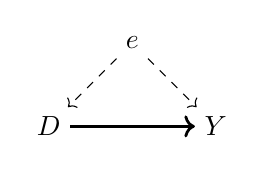
\begin{tikzpicture}
			[node distance=1.5cm]
		% nodes %
		\node[text centered] (e) {$e$};
		\node[below right of  = e, text centered] (y) {$Y$};
		\node[below left of = e, text centered] (d) {$D$};
 
		% edges %
		\draw[->, line width=1] (d) -- (y);
		\draw[dashed, ->] (e) -- (y);
		\draw[dashed, ->] (e) -- (d);
		\end{tikzpicture}
		\end{center}
		
		\begin{itemize}
		\item We are interested in the causal effect of juvenile incarceration ($D$) on life outcomes, like adult crime and high school completion
		\item But youth \emph{choose} to commit crimes, and that choice may be due to unobserved criminogenic factors like poverty or underlying criminal propensities which are themselves causing those future outcomes
		\end{itemize}
		

\end{frame}

\begin{frame}{Leniency as an instrument}

		\begin{center}
		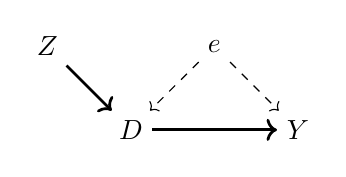
\begin{tikzpicture}
			[node distance=1.5cm]
		% nodes %
		\node[text centered] (e) {$e$};
		\node[below right of  = e, text centered] (y) {$Y$};
		\node[below left of = e, text centered] (d) {$D$};
		\node[above left of = d, text centered] (z) {$Z$};
 
		% edges %
		\draw[->, line width=1] (d) -- (y);
		\draw[->, line width=1] (z) -- (d);
		\draw[dashed, ->] (e) -- (y);
		\draw[dashed, ->] (e) -- (d);
		\end{tikzpicture}
		\end{center}
		
		\begin{itemize}
		\item Aizer and Doyle (2015) propose an instrument - the propensity to convict by the judge the youth is randomly assigned
		\item If judge assignment is random, and the various assumptions hold, then the IV strategy identifies the local average treatment effect of juvenile incarceration on life outcomes
		\end{itemize}

\end{frame}


\begin{frame}{The Main Idea}

	\begin{itemize}
	\item ``Plausibly exogenous'' variation in juvenile detention stemming from the random assignment of cases to judges who vary in their sentencing
	\item Consider two juveniles randomly assigned to two different judges with different incarceration tendencies (Scott and Bob)
	\item Random assignment ensures that differences in incarceration between Scott and Bob are due to the judge, not themselves, because remember, they're identical
	\end{itemize}
\end{frame}

\begin{frame}{Data}

	\begin{itemize}
	\item 35,000 juveniles administrative records over 10 years who came before a juvenile court in Chicago (Juvenile Court of Cook County Delinquency Database)
	\item Data were linked to public school data for Chicago (Chicago Public Schools) and adult incarceration data for Illinois (Illinois Dept. of Corrections Adult Admissions and Exits)
	\item They wanted to know the effect of juvenile incarceration on high school completion (2nd data needed) and adult crime (3rd data needed) using randomized judge assignment (1st data needed)
	\item They need personal identifying information in each data set to make this link (i.e., name, DOB, address)
	\end{itemize}
	
\end{frame}

\begin{frame}{Preview of findings}

	\begin{itemize}
	\item Juvenile incarceration decreased high school graduation by 13 percentage points (vs. 39pp in OLS)
	\item Increased adult incarceration by 23 percentage points (vs. 41pp in OLS)
	\item Marginal cases are high risk of adult incarceration and low risk of high school completion as a result of juvenile custody
	\item Unlikely to ever return to school after incarcerated, but when they do return, they are more likely to be classified as special ed students, and more likely to be classified for special ed services due to behavioral/emotional disorders (as opposed to cognitive disability)
	\end{itemize}
	
\end{frame}

\begin{frame}{``Plausibly'' exogenous}

	\begin{itemize}
	\item Very common in these studies for the assignment to some decision-maker to be \emph{arbitrary} but not clearly random (i.e., not random no. generator)
	\item In this case, juveniles charged with a crime are assigned to a calendar corresponding to their neighborhood and calendars have 1-2 judges who preside over them
	\item 1/5 of hearings are presided over by judges who cover the calendar when the main judge can't, known as swing judges
	\item Judge assignment is a function of the sequence with which cases happen to enter into the system and judge availability that is set in advance
	\item No scope for which judge you see first; conversations with court administrators confirm its random
	\end{itemize}
\end{frame}

\begin{frame}{Structural equation}

\begin{eqnarray*}
Y_i = \beta_0 + \beta_1 JI_i + \beta_2 X_i + \varepsilon_i
\end{eqnarray*}where $X_i$ is controls and $\varepsilon_i$ is an error term.  In this, juvenile incarceration is likely correlated with the error term.

\bigskip

This is the ``long'' causal model. But note, from the prior DAG, we cannot control for $e$ because it is unobserved. But it is confounding the estimation of juvenile incarceration's effect on outcomes.

\end{frame}

\begin{frame}{Incarceration Propensity as an Instrument}

	\begin{itemize}
	\item The instrument is based on the randomized judge equalling the propensity to incarcerate from the randomly assigned judge
	\item ``Leave-one-out mean''$$Z_{j(i)} = \bigg ( \frac{1}{n_{j(i)} - 1} \bigg ) \bigg ( \sum_{k \neq i}^{n_{j(i)}-1} \widetilde{JI}_k \bigg )$$
	\item The $n_{j(i)}$ terms is the total number of cases seen by judge $k$, and $\widetilde{JI}_k$ is equal to 1 if the juvenile was incarcerated during their first case
	\item Thus the instrument is the judge's incarceration among first cases based on all their other cases
	\item It's basically a judge fixed effect given the likelihood two judges have precisely the same propensity is small
	\end{itemize}
\end{frame}

\begin{frame}{Information about the instrument}

\begin{itemize}
	\item There are 62 judges in the data, and the average number of initial cases per judge is 607
	\item Substantial variation in the data - raw measure ranges from 4\% to 21\%
	\item Residualized measure based on controls still has substantial variation from 6\% to 18\%
	\item Variation comes from two sources: variation among the regular (nonswing) judges (80\% of cases) and variation from the swing judges (20\% of cases)
\end{itemize}

\end{frame}

\begin{frame}{Distribution of IV}
	
	\begin{figure}
	\includegraphics[scale=0.15]{./lecture_includes/iv.png}
	\end{figure}
\end{frame}
	
\begin{frame}{Balance test}
	
	\begin{figure}
	\includegraphics[scale=0.15]{./lecture_includes/balance.png}
	\end{figure}
\end{frame}

\begin{frame}{First stage}
	
	\begin{figure}
	\includegraphics[scale=0.15]{./lecture_includes/firststage.png}
	\end{figure}
\end{frame}


\begin{frame}{High school completion}
	
	\begin{figure}
	\includegraphics[scale=0.15]{./lecture_includes/highschool.png}
	\end{figure}
\end{frame}


\begin{frame}{Adult crime}
	
	\begin{figure}
	\includegraphics[scale=0.2]{./lecture_includes/adult_crime.png}
	\end{figure}
\end{frame}


\begin{frame}{Crime type}
	
	\begin{figure}
	\includegraphics[scale=0.2]{./lecture_includes/crimetype.png}
	\end{figure}
\end{frame}


\begin{frame}{High school transfers}
	
	\begin{figure}
	\includegraphics[scale=0.2]{./lecture_includes/transfers.png}
	\end{figure}
\end{frame}


\begin{frame}{Developing emotional problems}
	
	\begin{figure}
	\includegraphics[scale=0.2]{./lecture_includes/disorder.png}
	\end{figure}
\end{frame}


\begin{frame}{Concluding remarks}

	\begin{itemize}
	\item Identifying causal effect without an instrument is likely not possible given the deep selection issues associated with crime as a child and adult
	\item Leniency designs are everywhere, even in tech, but you need to know how to look for them
	\item Bottleneck, influential decision-makers, discretion - these are the three elements of the design
	\end{itemize}

\end{frame}


\subsection{Price elasticity of demand}

\begin{frame}{Supply and Demand}

\begin{itemize}
\item Instrumental variables was developed in the 1920s largely to address problems created by supply and demand
\item Demand curves are causal functions, but so are supply curves
\item We do not observe all the prices and quantities to be able to calculate the slope or shape of the demand curve because we only observe the ``realized prices and quantities'' in equilibrium
\item But if we did know the price elasticity of demand, we could set more optimal policies like tax policy or profit maximization
\end{itemize}

\end{frame}

\begin{frame}{Supply and Demand}
	
	\begin{figure}
	\includegraphics[scale=0.72]{./lecture_includes/supply_demand.pdf}
	\end{figure}
\end{frame}


\begin{frame}{Initial price and quantity}

	\begin{figure}
	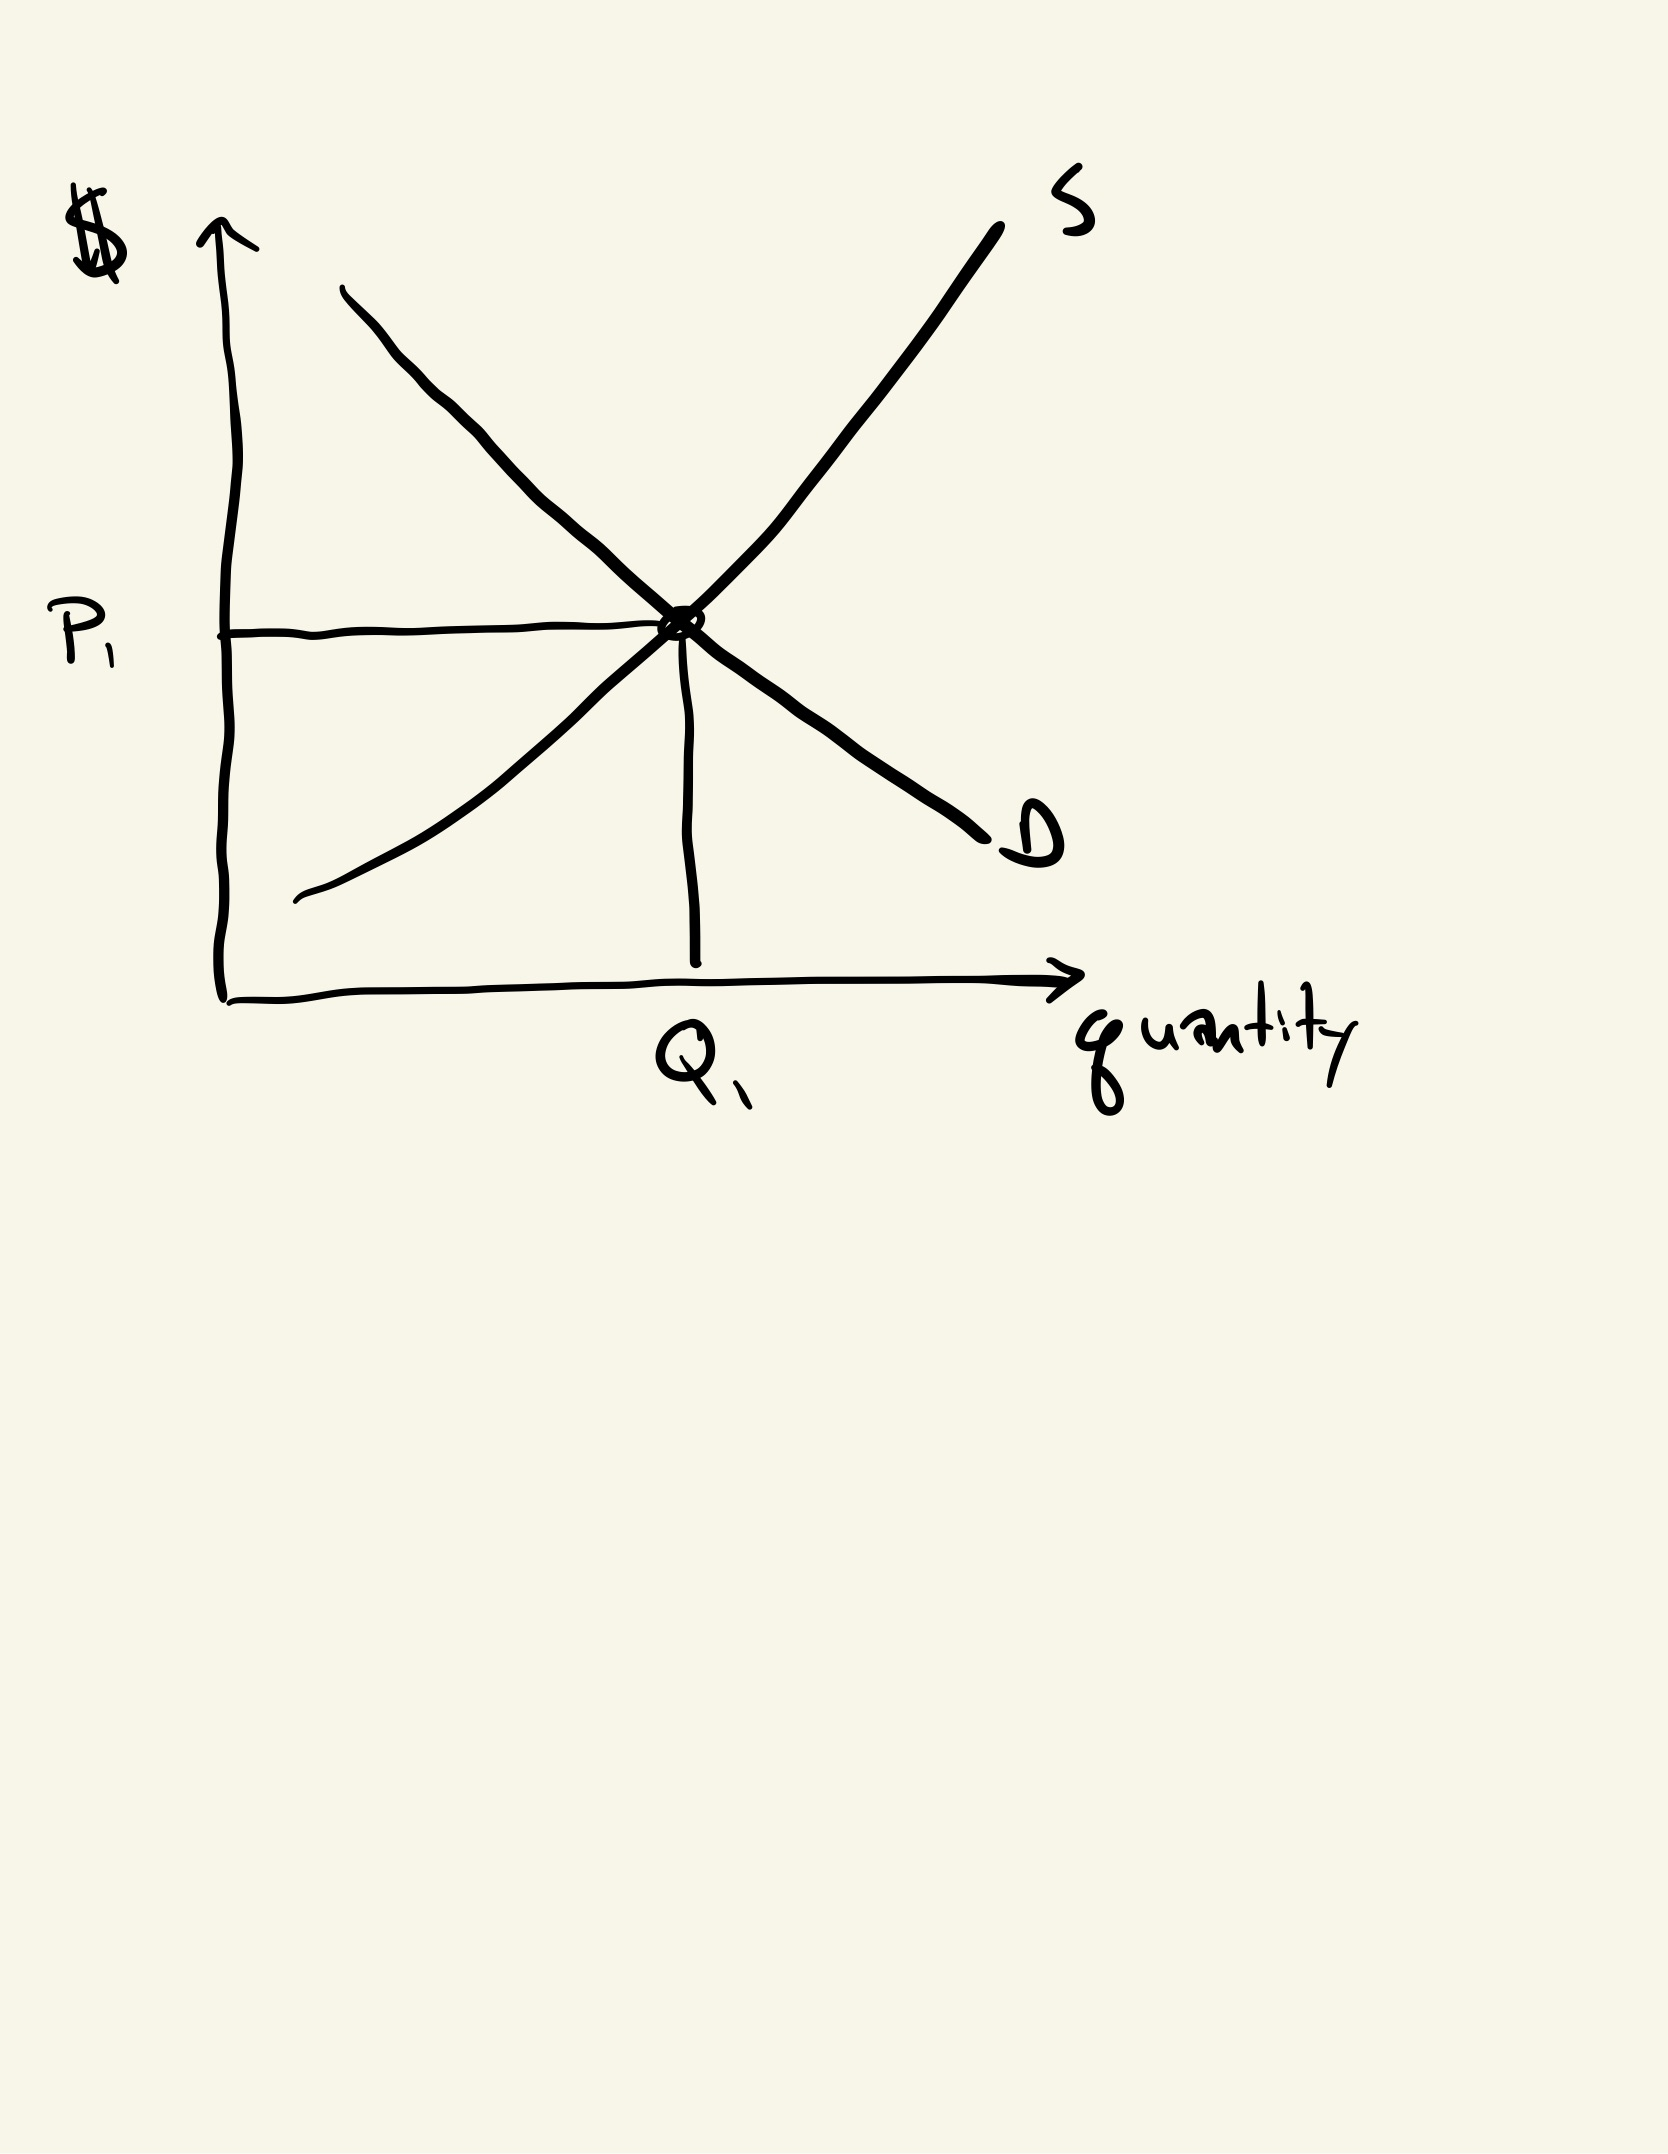
\includegraphics[scale=0.15]{./lecture_includes/elasticity_1.jpg}
	\end{figure}
\end{frame}

\begin{frame}{Supply shift}

	\begin{figure}
	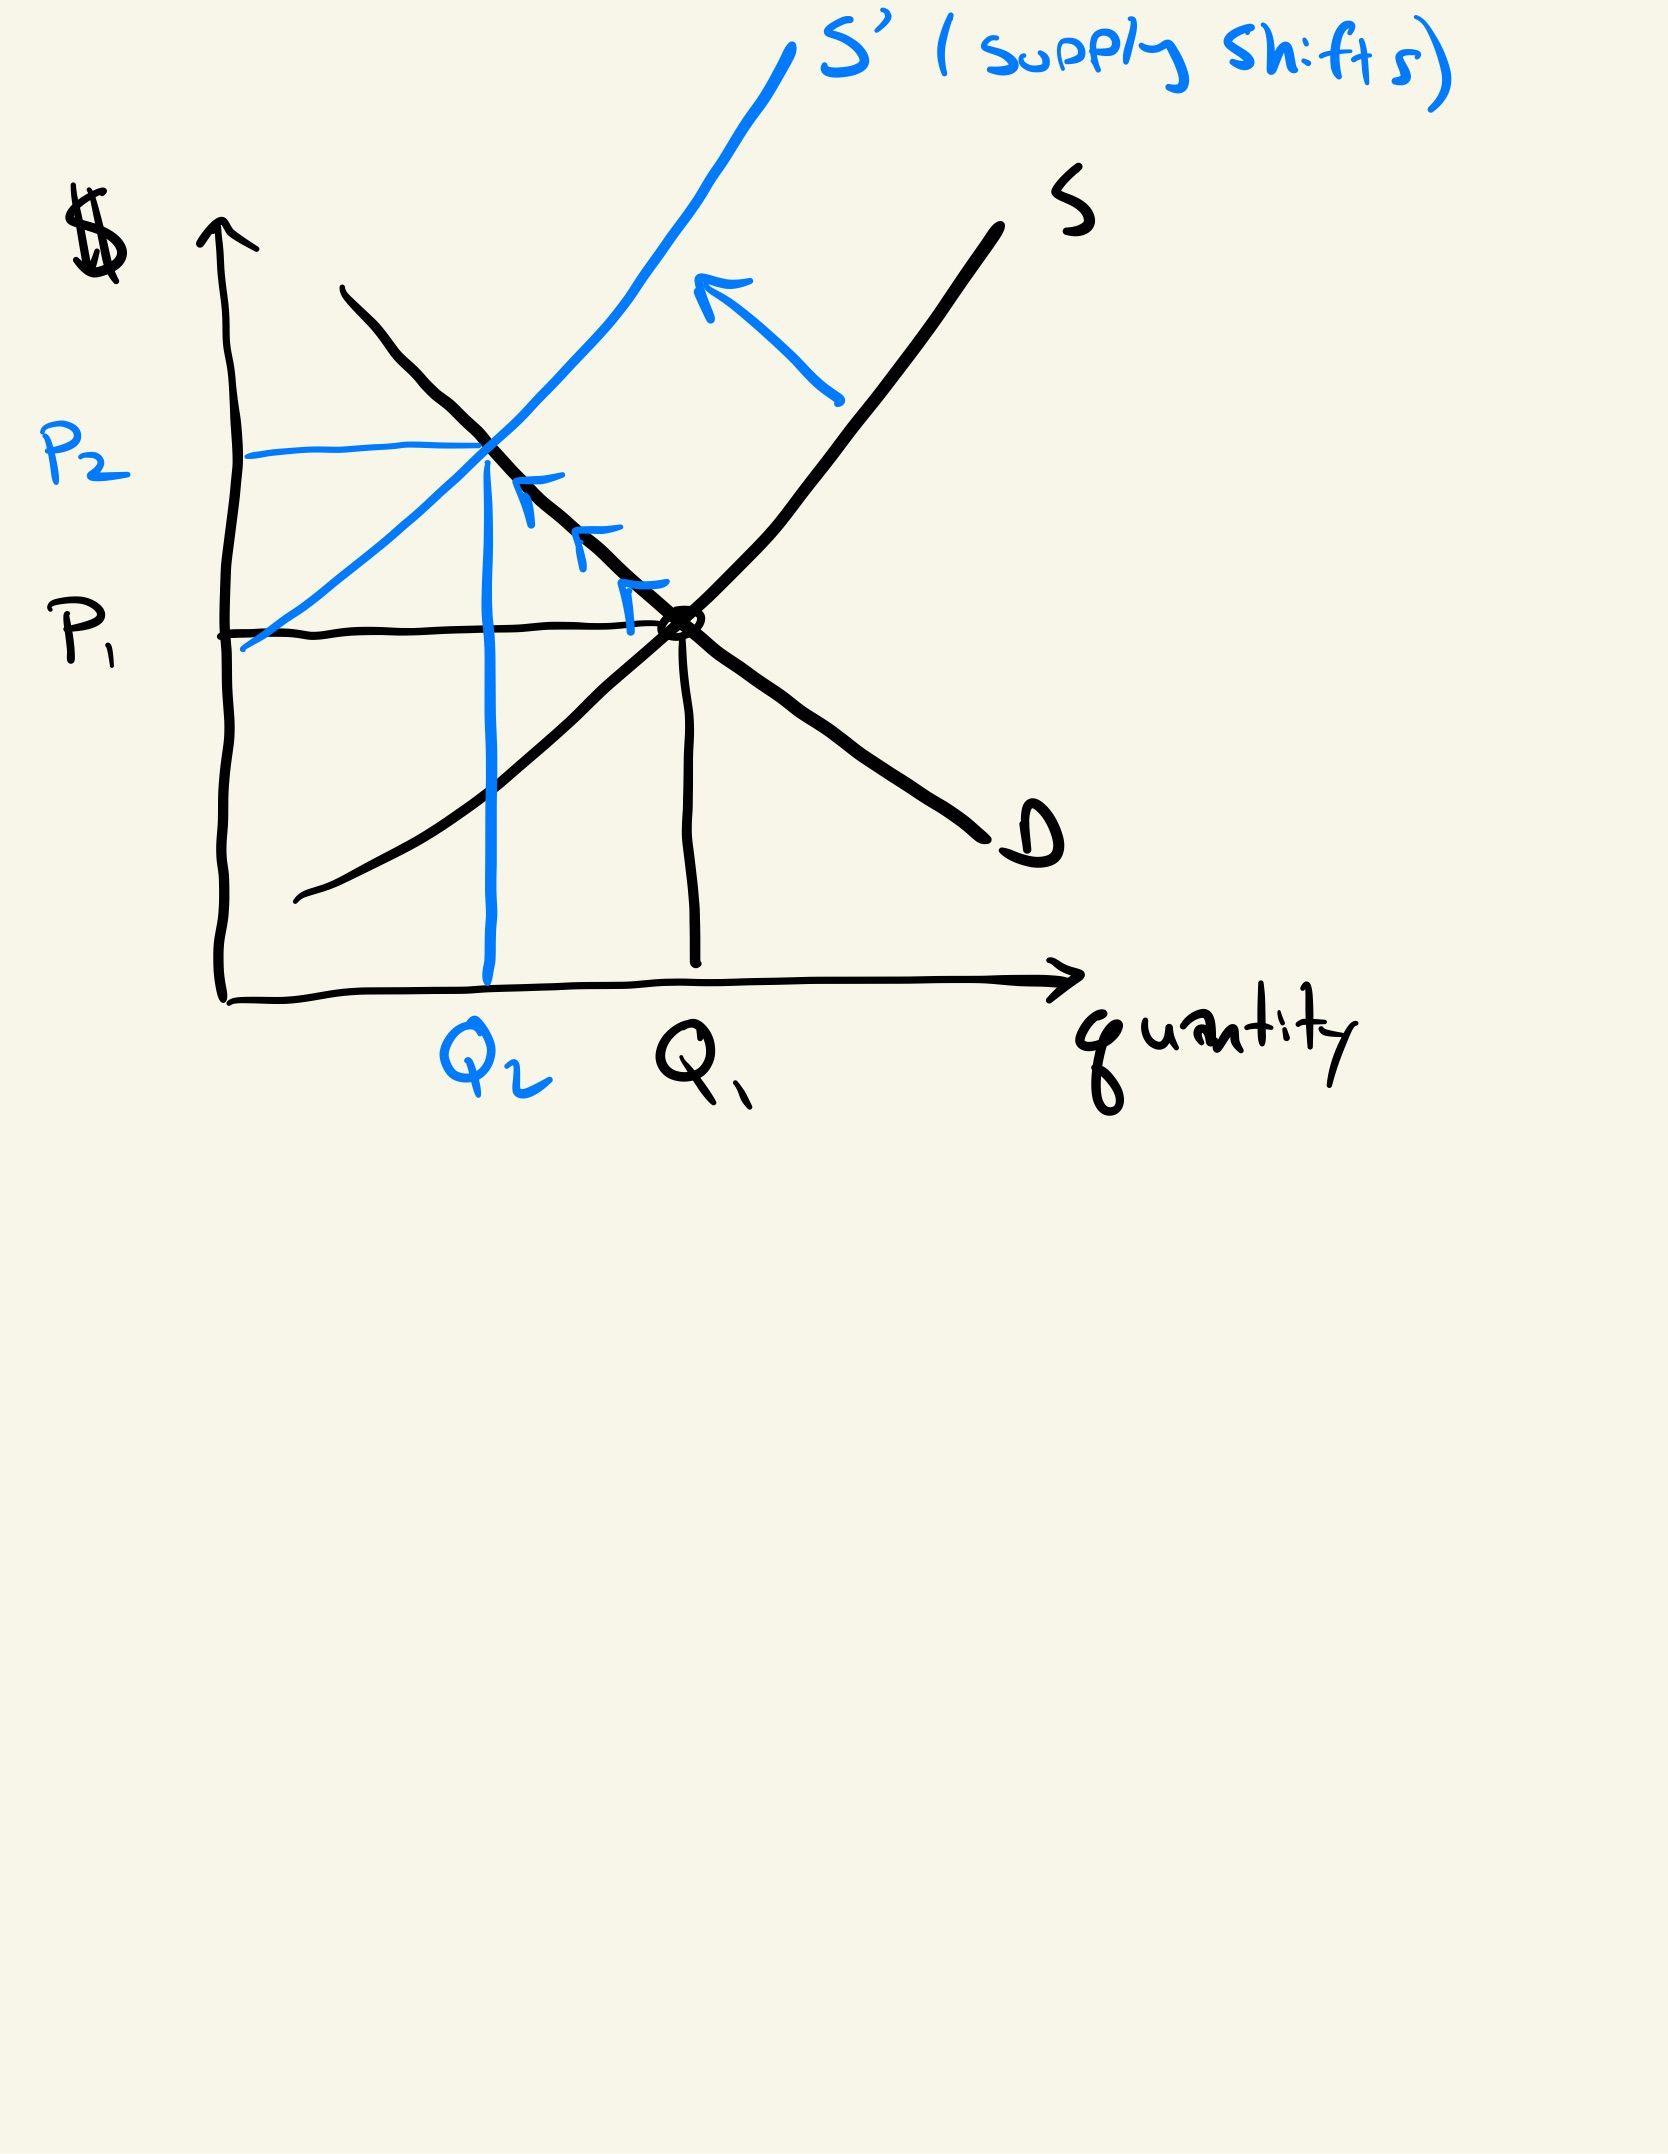
\includegraphics[scale=0.15]{./lecture_includes/elasticity_2.jpg}
	\end{figure}
\end{frame}


\begin{frame}{Price elasticity of demand}

\begin{eqnarray*}
\delta = \frac{Q_2 - Q_1}{P_2 - P_1}
\end{eqnarray*}

\bigskip

Can be estimated with log-log regressions:

\bigskip

\begin{eqnarray*}
Ln Q_{it} = \alpha + \delta Ln P_{it} + \psi_{it}
\end{eqnarray*}

\bigskip

But you need an instrument for price and it must be a supply shifter only


\end{frame}

\begin{frame}{Supply shift}

\begin{itemize}
\item \textbf{Supply shifters}: Firm input costs and technology are typical candidates
\item \textcolor{red}{Demand shifters}: Other consumer good prices, consumer income, availability of substitutes, expectations about the future
\item Good instruments must shift \textbf{only} supply -- \textcolor{red}{not demand}
\end{itemize}

\end{frame}

\begin{frame}{Elasticity of meth demand}

	\begin{figure}
	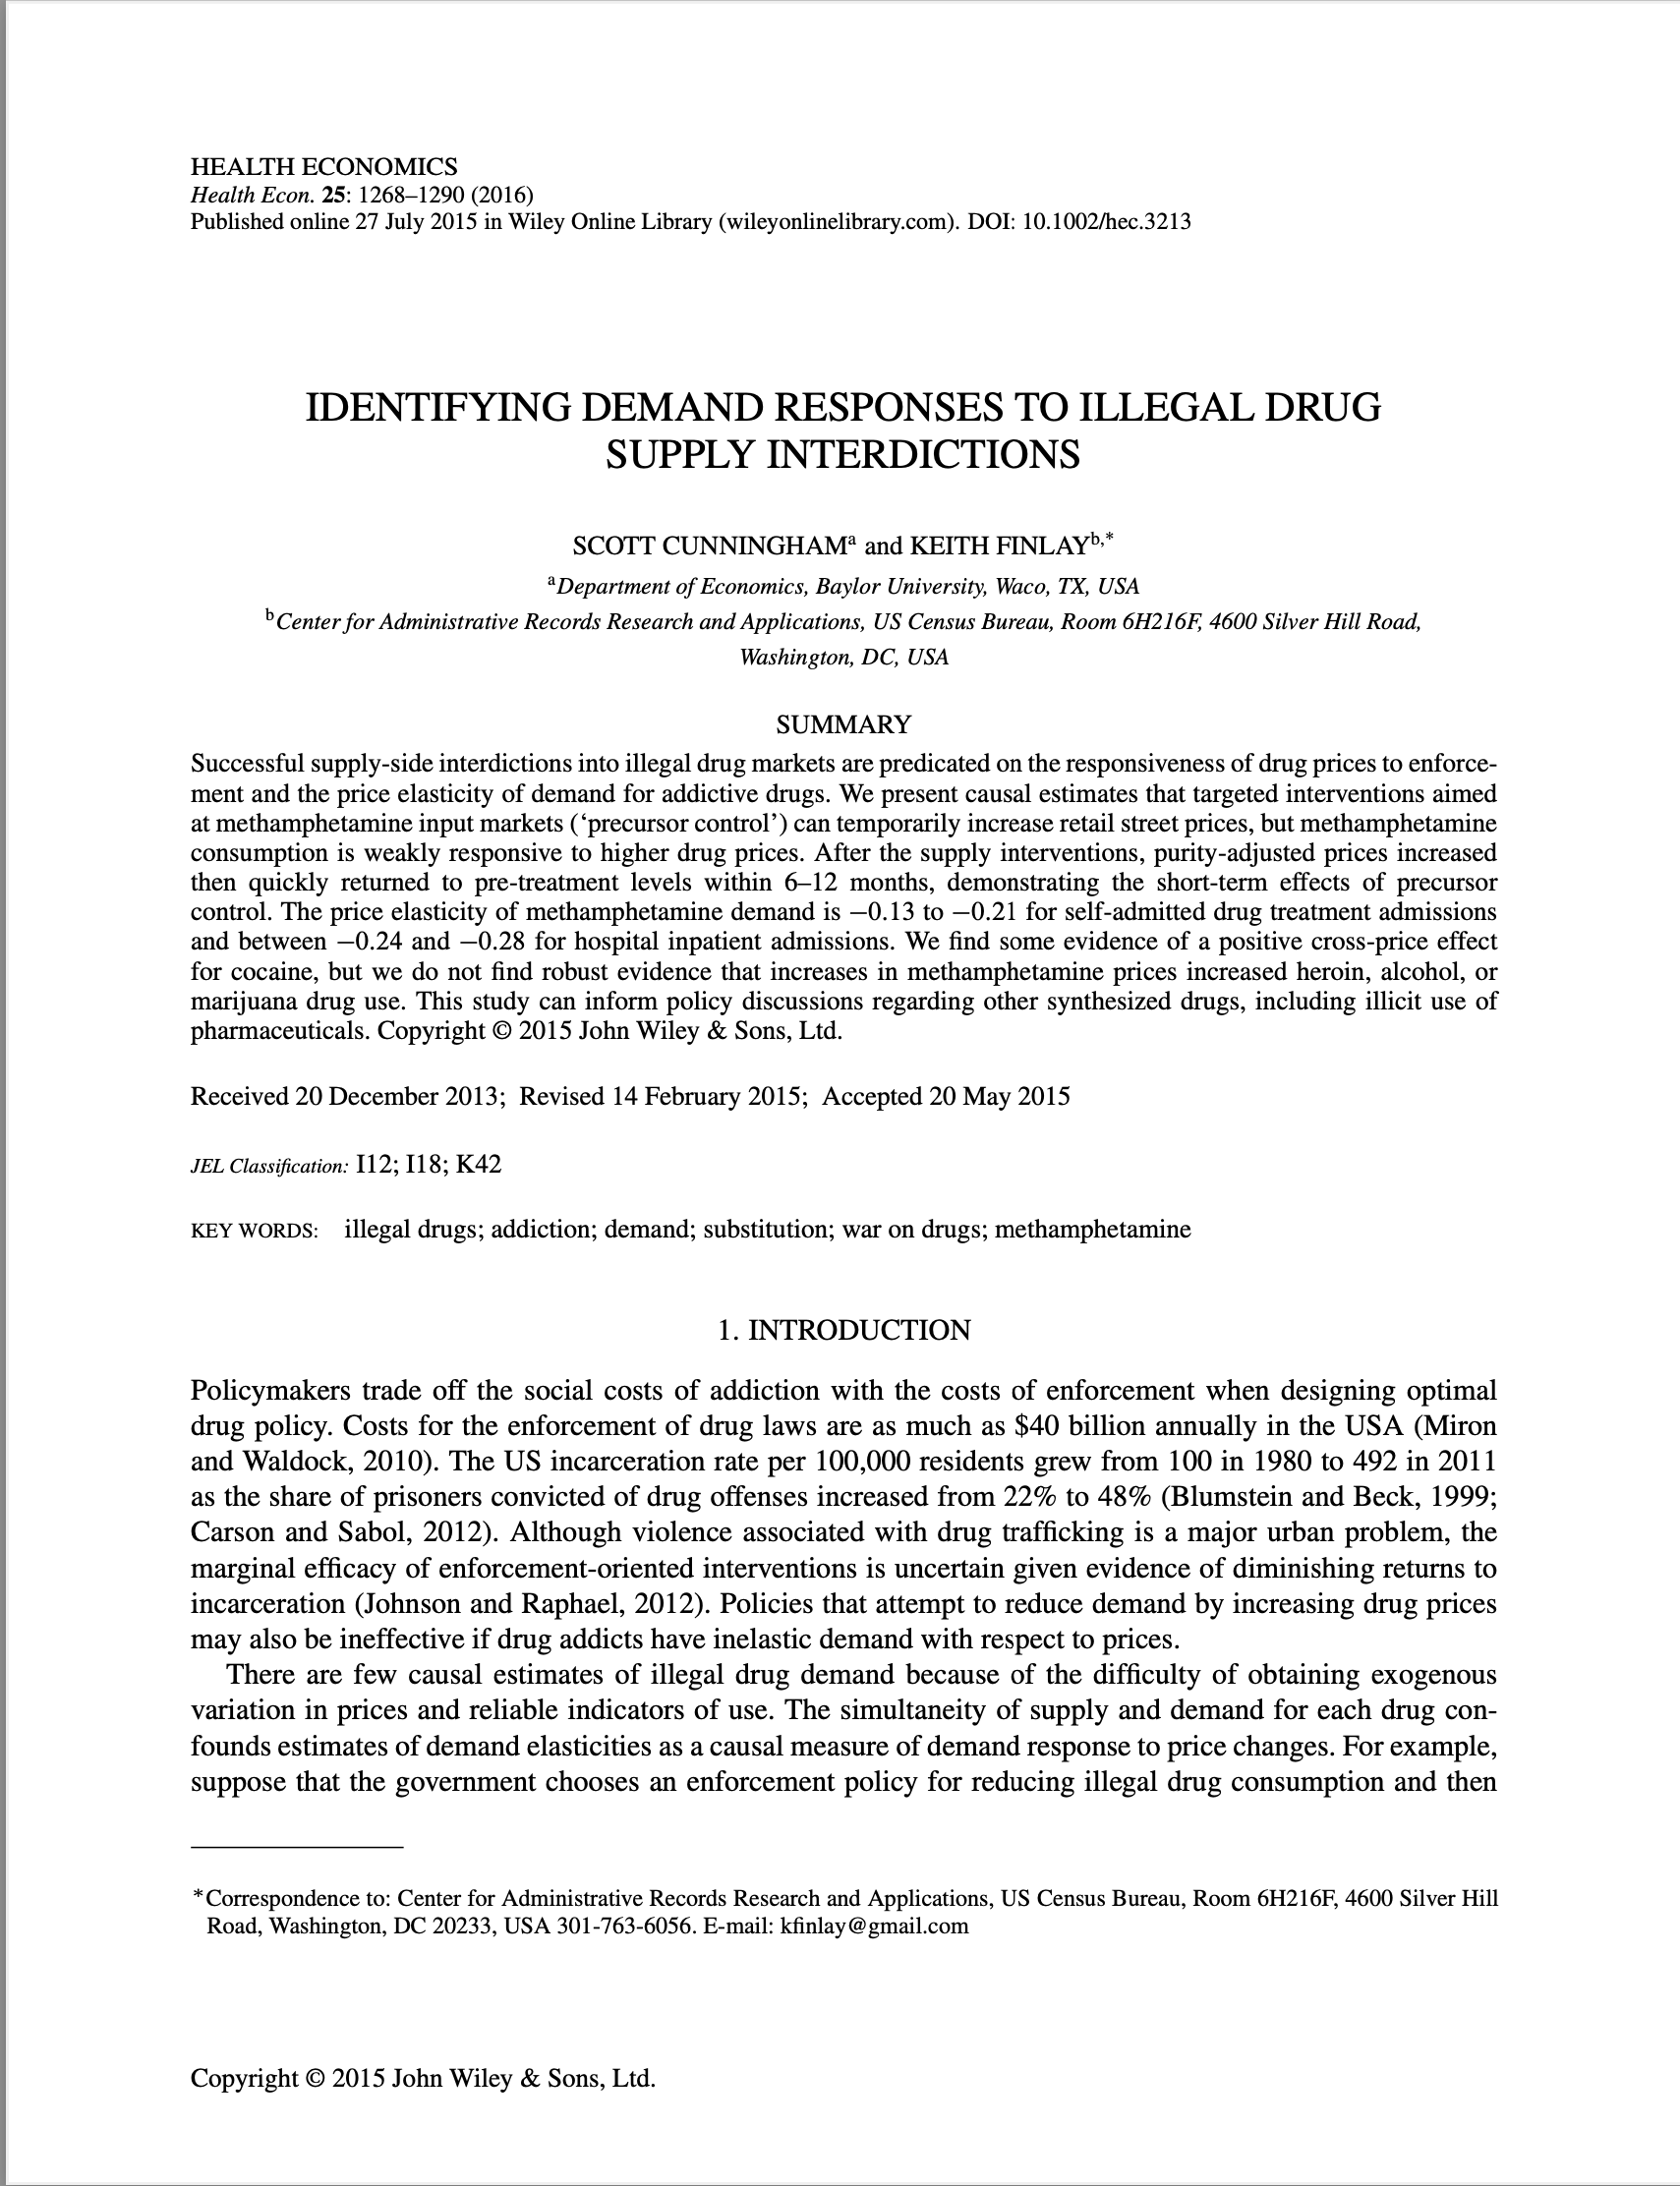
\includegraphics[scale=0.25]{./lecture_includes/he_1}
	\end{figure}
\end{frame}

\begin{frame}{Cooking meth}

\begin{itemize}
\item d-methamphetamine is a chemical product synthesized from either ephedrine or pseudoephedrine 
\item 1995, 1997 and 2003 there were several federal regulations that restricted access to these precursors as an effort combat meth epidemic
\item Undercover meth seizure data showed massive increases in real price of meth on the street in response
\end{itemize}

\end{frame}

\begin{frame}{Meth purity plummetted}

	\begin{figure}
	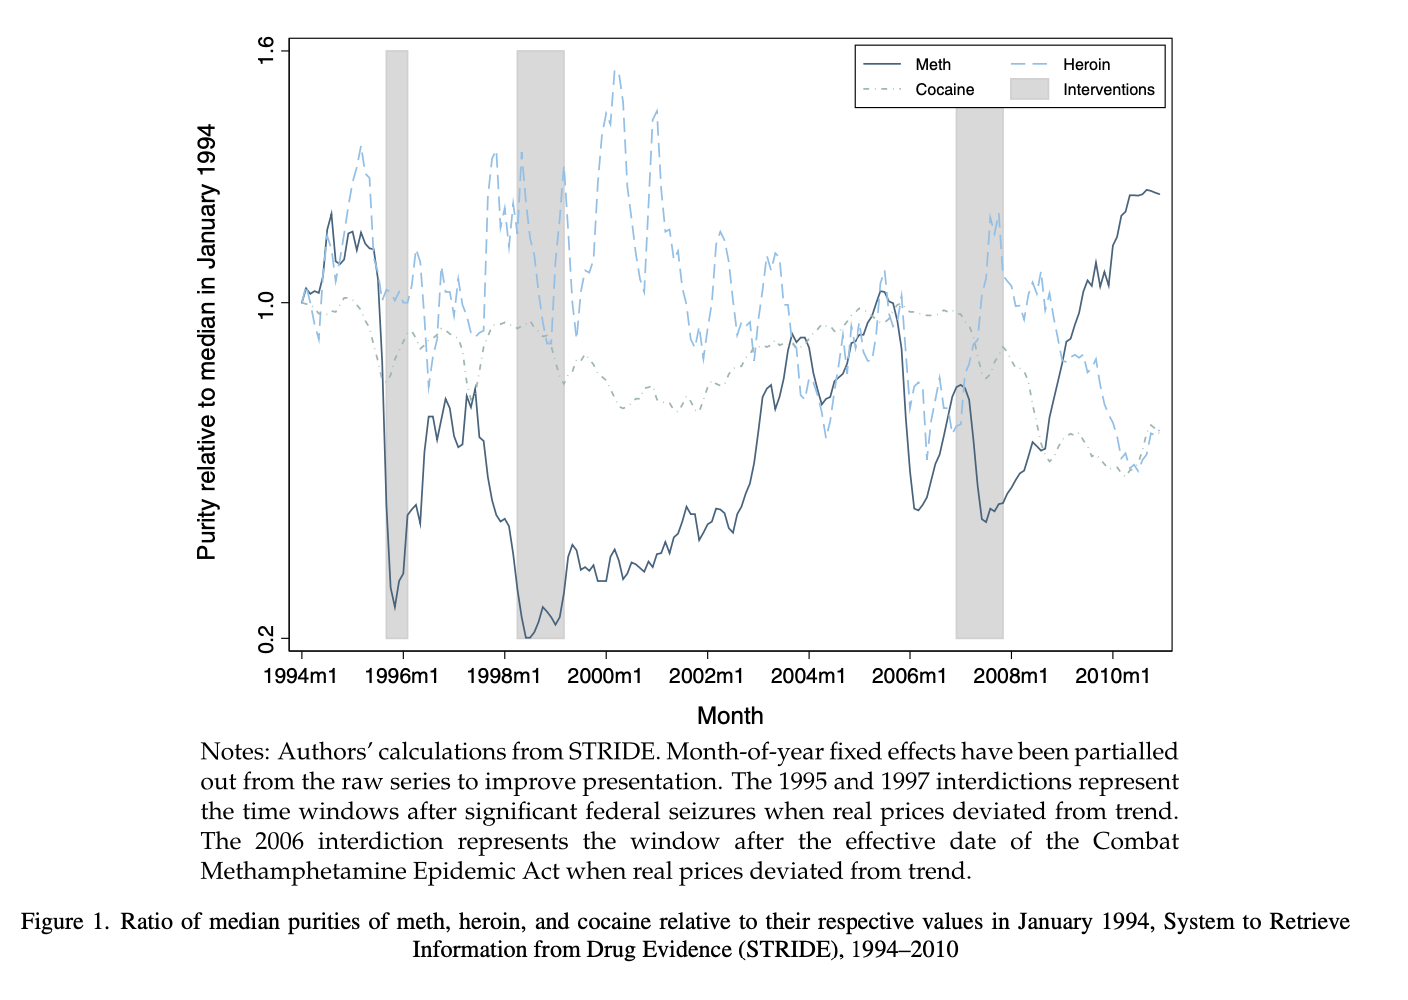
\includegraphics[scale=0.35]{./lecture_includes/he_2}
	\end{figure}
\end{frame}

\begin{frame}{Meth prices skyrocketed}

	\begin{figure}
	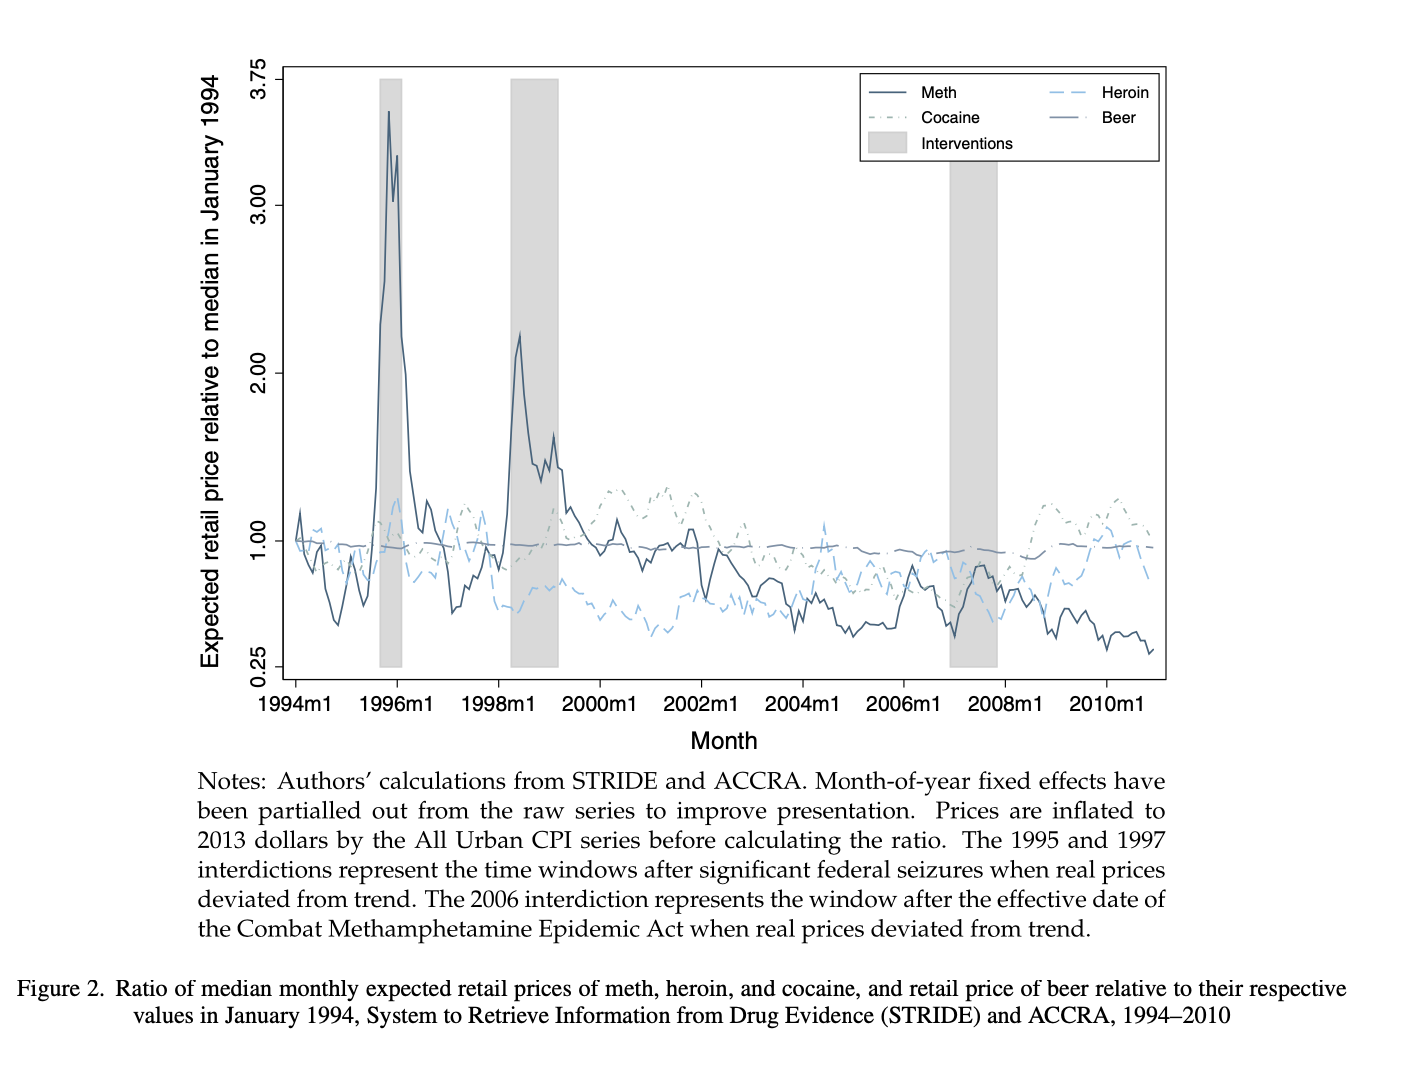
\includegraphics[scale=0.35]{./lecture_includes/he_3}
	\end{figure}
\end{frame}

\begin{frame}{Meth admissions to treatment and hospitals fell}

	\begin{figure}
	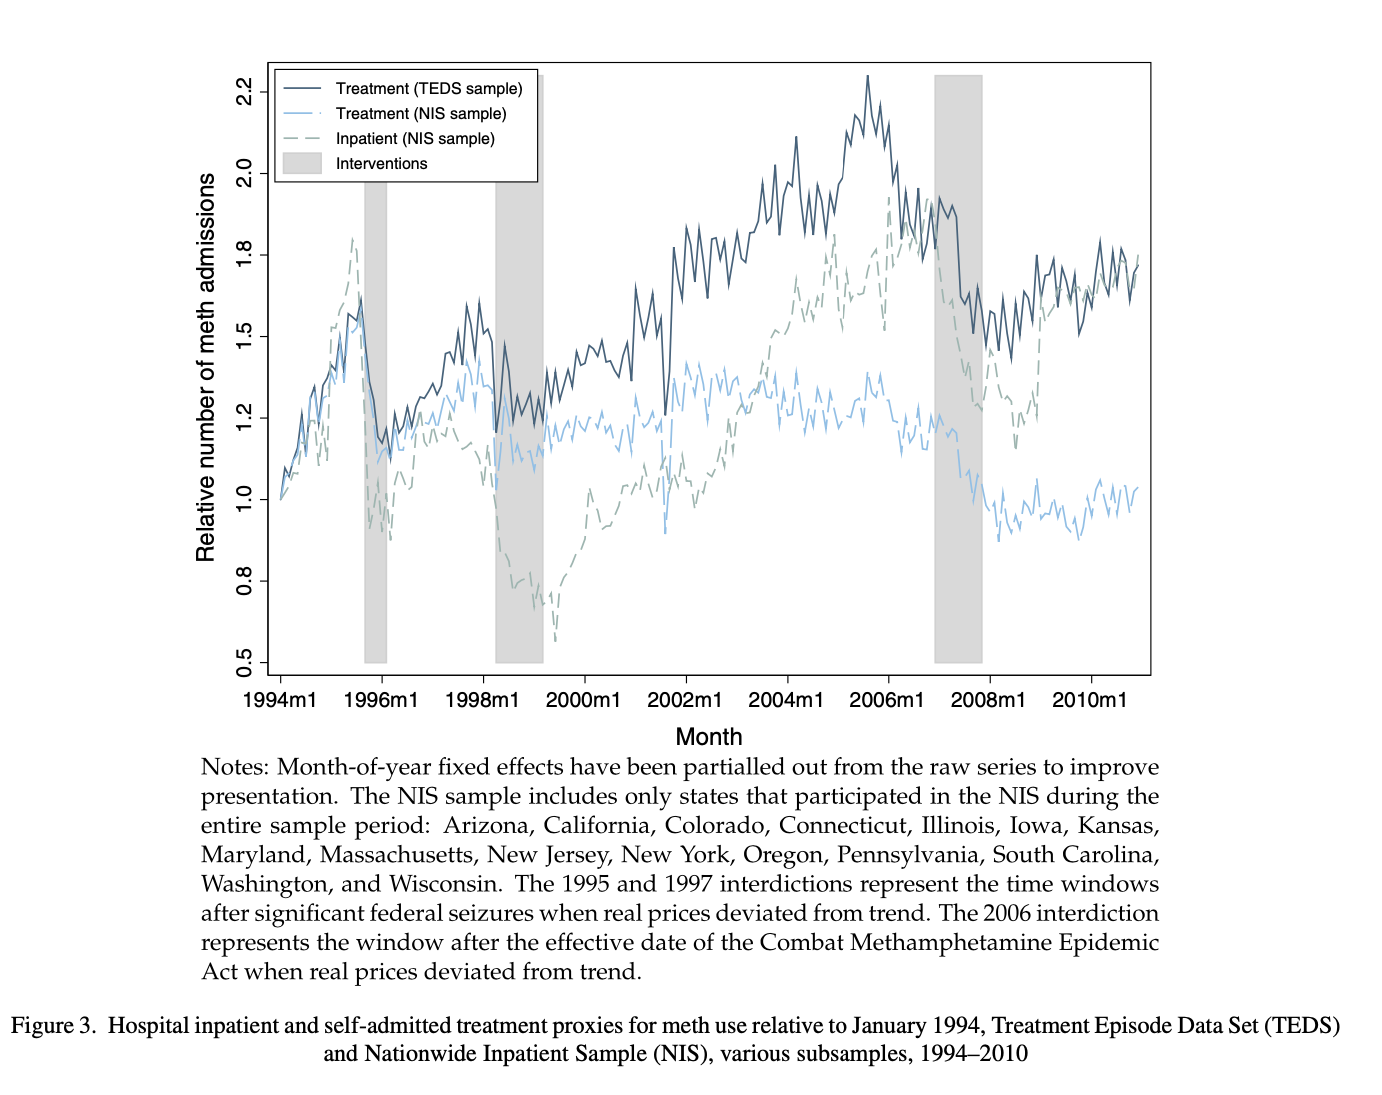
\includegraphics[scale=0.35]{./lecture_includes/he_4}
	\end{figure}
\end{frame}


\begin{frame}{OLS and 2SLS Estimation}

	\begin{figure}
	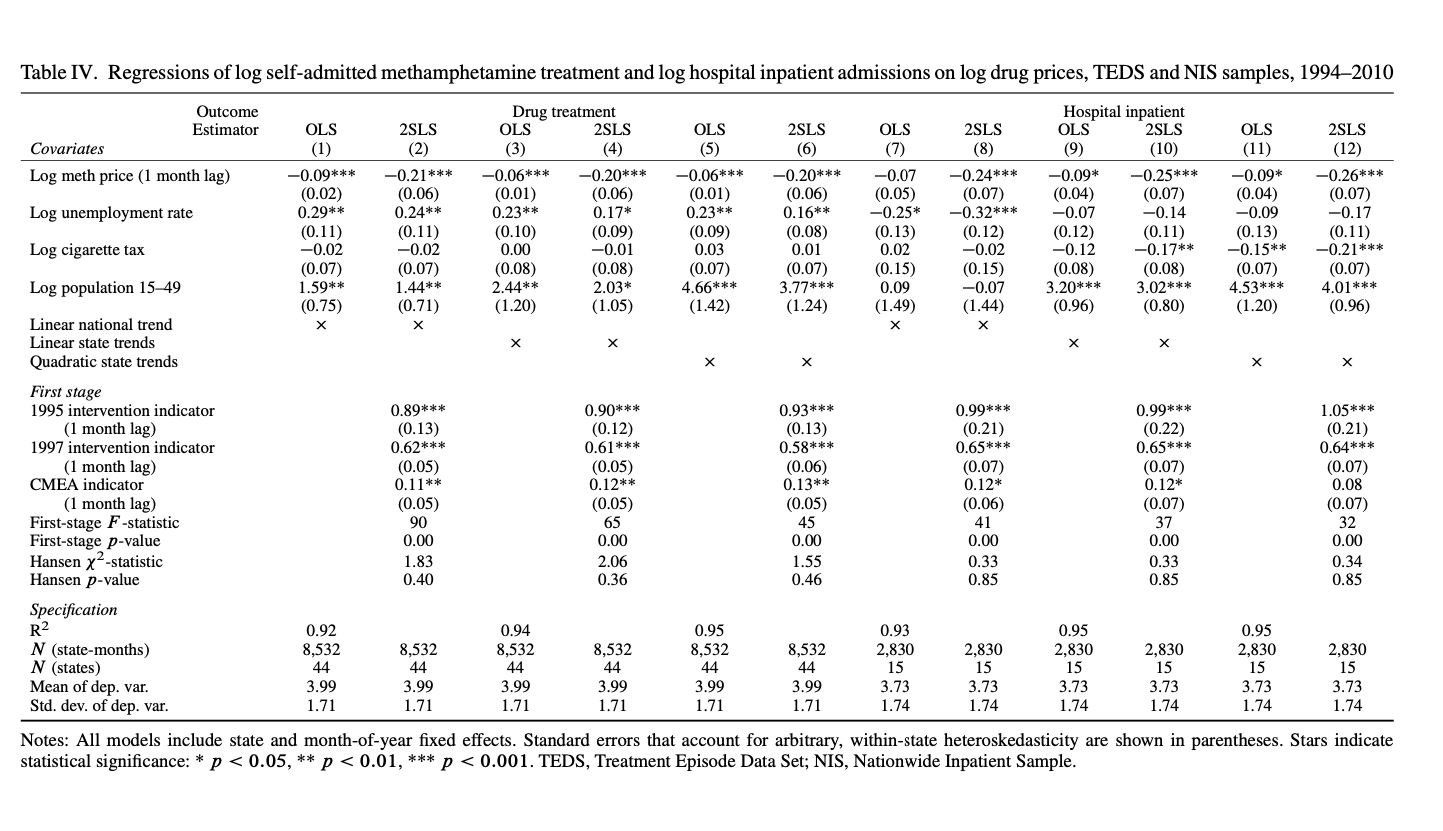
\includegraphics[scale=0.35]{./lecture_includes/he_7}
	\end{figure}
\end{frame}

\begin{frame}{Discussion}

\begin{itemize}
\item Highly inelastic (-0.21 to -0.26) and robust across two measures of meth consumption
\item Need data on prices and quantities, required FOIA requests to Drug Enforcement Agency and purchasing data on hospitalizations and treatment
\item But crucially needed something that would've raised firm costs through inputs that was not related to consumer demand (theory guided)
\item Instruments were deviations in the price from longterm trends
\end{itemize}

\end{frame}

\begin{frame}{Discussion}

\begin{itemize}
\item There are other ways to estimate demand, but this method is one that should immediately be exploited when supply shocks happen
\item Focus needs to be on inputs for which there are not instantly the ability to substitute
\item But can't be so correlated with broader demand shocks that you are back shifting supply and demand (e.g., COVID)
\end{itemize}

\end{frame}

\section{Conclusion}

\begin{frame}{Conclusion}

\begin{itemize}
\item ``With a long enough lever, I can move the world'' -- Archimedes
\item With a strong enough and strange enough instrument, you can identify the LATE even outside of the laboratory
\item Need to know what to look for so keep that DAG in mind all the time -- write it on the wall
\item But like selection on observables, we need plausible assumptions, properly measured data and appropriate estimators
\end{itemize}

\end{frame}


\end{document}



\subsection{Leniency design}


\begin{frame}{Comments on judge fixed effects}

\begin{itemize}
	\item Leave-one-out average propensity of the decision-maker, or some residualized instrument, is very common
	\item More often you'll see jackknife IV (JIVE) which drops observations while running regressions to improve finite sample bias
	\item The biggest threats aren't exclusion probably (though sometimes), but monotonicity
	\item Might judges be harsh in some situations (violent crimes) but lenient in others (female defendants, first time offenders)
\end{itemize}

\end{frame}

\begin{frame}{Tests for violations}

\begin{itemize}
\item New paper by Frandsen, Lefgren and Leslie (2019) proposes a test 
\item They show that the identifying assumptions imply a conditional expectation of the outcome of interest given the judge assignment is a continuous function of the judge propensity 
\item They propose a two-part test that generalizes the Sargan-Hansen over identification test and assesses whether treatment effects across judge propensities are possible 
\item Software available on Emily Leslie's website
\end{itemize}

\end{frame}

\begin{frame}{Multi-dimensional instrument}

\begin{itemize}
\item Peter Hull in a cautionary note notes that while combining judge fixed effects into a single propensity is numerically equivalent, it's still a series of dummies
\item Therefore it's very important to keep in mind the lessons we learned from weak instruments -- the more weak instruments you have when a parameter is overidentified, the larger the bias
\item It's ongoing at the moment to think about ways to improve instrument selection, but not settled
\item I encourage you to read Peter's note on his website and begin thinking about this yourself
\end{itemize}

\end{frame}


\begin{frame}{Discussion questions}

\begin{itemize}
\item When working on a judge fixed effects project, write down an IV DAG 
\item Whereas monotonicity cannot be visualized to my knowledge on a DAG, exclusion can -- so what does an exclusion violation mean in this context?
\item Use logic and conversations with those administering the program to answer the following -- what does monotonicity mean in this context and how might it be violated?  
\end{itemize}

\end{frame}


\begin{frame}{Empirical exercise}

\begin{itemize}

\item Let's estimate the effect of cash bail on defendant outcomes using 2SLS and JIVE
\item Excellent paper by Megan Stevenson
\item -\texttt{bail.do}- and -\texttt{bail.r}- in dropbox and github
\end{itemize}

\end{frame}





\begin{frame}{Phillip Wright}
	
	\begin{itemize}
	\item Philip Wright was a renaissance man - published in JASA, QJE, AER, you name it, while on a very intense teaching load. 
	\item Also published poetry, and even personally published Carl Sandburg's first book of poetry!
	\item Spent a long time at Tufts
	\item He was very concerned about the negative effects of tariffs and wrote a book about commodity markets
	\end{itemize}

\end{frame}

\begin{frame}{Elasticity of demand is unidentified}
	
	\begin{itemize}
	\item James Stock notes that his publications had a theme regarding identification
	\item He knew, for instance, that he couldn't simple look at correlations between price and quantity if he wanted the elasticity of demand due to simultaneous shifts in supply and demand
	\item The pairs of quantity and price weren't demand, or supply - they were demand and supply equilibrium values and therefore didn't reflect the demand or the supply curve, both of which are counterfactuals
	\item Those points are nothing more than a bunch of numbers -- no more, no less -- that have no practical use, scientific or otherwise
	\end{itemize}
	
\end{frame}

\begin{frame}[plain]

 \begin{figure}[h]
\includegraphics[scale=0.75]{./lecture_includes/supply_demand.pdf}
\caption{Wright's graphical demonstration of the identification problem}
\label{fig:sd}
\end{figure}

\end{frame}

\begin{frame}{Sewell Wright}

\begin{itemize}
\item Sewell was his son, who did \emph{not} go into the family business
\item Rather, he decided to become a genius and invent genetics
\item Developed path diagrams (which Pearl revived 50 years later for causal inference) 
\item Father and son engage in letter correspondence as Philip tried to solve the ``identification problem''

\end{itemize}

\end{frame}

\begin{frame}[plain]


\centering
  \begin{overprint}%
\begin{figure}[h]
  \makebox[\textwidth][c]{\includegraphics[width=1.0\textwidth]{./lecture_includes/wright_letter.png}}%
\caption{Wright's letter to Sewell, his son}
\end{figure}
  \end{overprint}%

\end{frame}


\begin{frame}[plain]


\centering
  \begin{overprint}%
\begin{figure}[h]
  \makebox[\textwidth][c]{\includegraphics[width=1.0\textwidth]{./lecture_includes/path_diagrams_wrights.png}}%
\caption{Recognize these?}
\end{figure}
  \end{overprint}%

\end{frame}


\begin{frame}{QJE Rejects}

\begin{itemize}
\item QJE misses a chance to make history and rejects his paper proving an IV estimator
\item Sticks his proof in Appendix B of 1928 book, \underline{The Tariff on Animal and Vegetable Oils}
\item His work on IV is ignored, and is then rediscovered 15 years later (e.g., Olav Reiers\o l). 
\item James Stock and others have helped correct the record
\end{itemize}

\end{frame}


\begin{frame}{Sidebar: stylometric analysis}

\begin{itemize}
\item Long standing question was who \emph{wrote} Appendix B? Answer according to Stock and Trebbi (2003) using stylometric methods is that Philip \emph{wrote} it.
\item But who invented it?  It was collaborative, but Sewell acknowledged he didn't know how to handle endogeneity and simultaneity (that was Philip)
\end{itemize}

\end{frame}


\subsection{Lottery designs}


\begin{frame}{IV in Randomized Trials}
	
	\begin{itemize}
	\item In many randomized trials, participation is nonetheless voluntary among those randomly assigned to treatment
	\item Consequently, noncompliance is not uncommon and without correcting for it, creates selection biases
	\item IV designs may even be helpful when evaluating a randomized trial, even though treatment was randomly assigned
	\item The solution is to instrument for treatment with whether you ``won the lottery'' and estimate LATE
	\end{itemize}
	
\end{frame}

	
\begin{frame}{Lottery designs}
	
	\begin{itemize}
	\item The instrument is your randomized lottery
	\item Examples might be randomized lottery for attending charter schools to study effect of charter schools on educational outcomes, or a randomized voucher to encourage the collection of health information
	\item Recall Thornton (2008) instrumented for getting HIV results to estimate causal effect of learning one was HIV+ on condom purchases
	\item We'll discuss two papers from 2012 and 2014 evaluating a lottery-based expansion of Medicaid health insurance on Oregon on numerous health and financial outcomes
	\end{itemize}
\end{frame}


\begin{frame}{Overarching question}
	
	\begin{itemize}
	\item What are the effects of expanding access to public health insurance for low income adults?
		\begin{itemize}
		\item Magnitudes, and even the signs, associated with that question were uncertain
		\end{itemize}
	\item Limited existing evidence
		\begin{itemize}
		\item Institute of Medicine review of evidence was suggestive, but a lot of uncertainty
		\item Observational studies are confounded by selection into health insurance
		\item Quasi-experimental work often focuses on elderly and children
		\item Only one randomized experiment in a developed country: the RAND health insurance experiment
			\begin{itemize}
			\item 1970s experiment on a general population
			\item Randomized cost-sharing, not coverage itself
			\end{itemize}
		\end{itemize}
	\end{itemize}
\end{frame}



\begin{frame}{The Oregon Health Insurance Experiment}
	
	 Setting: Oregon Health Plan Standard
		\begin{itemize}
		\item Oregon's Medicaid expansion program for poor adults
		\item Eligibility
			\begin{itemize}
			\item Poor ($<$100\% federal poverty line) adults 19-64
			\item Not eligible for other programs
			\item Uninsured $>$ 6 months
			\item Legal residents
			\end{itemize}
		\item Comprehensive coverage (no dental or vision)
		\item Minimum cost-sharing
		\item Similar to other states in payments, management 
		\item Closed to new enrollment in 2004
		\end{itemize}
\end{frame}



\begin{frame}{The Oregon Medicaid Experiment}
	
Oregon held a lottery
		\begin{itemize}
		\item Waiver to operate lottery
		\item 5-week sign-up period, heavy advertising (January to February 2008)
		\item Low barriers to sign up, no eligibility pre-screening
		\item Limited information on list
		\item Randomly drew 30,000 out of 85,000 on list (March-October 2008)
		\item Those selected given chance to apply
			\begin{itemize}
			\item Treatment at household level
			\item Had to return application within 45 days
			\item 60\% applied; 50\% of those deemed eligible $\rightarrow$ 10,000 enrollees 
			\end{itemize}
		\end{itemize}
\end{frame}

\begin{frame}{Oregon Health Insurance Experiment}
	
	\begin{itemize}
	\item Evaluate effects of Medicaid using lottery as randomized controlled trial (RCT)
		\begin{itemize}
		\item Intent-to-treat: Reduced form comparison of outcomes between treatment group (lottery selected individuals) and controls (not selected)
		\item LATE: IV using lottery as instrument for insurance coverage
			\begin{itemize}
			\item First stage: about a 25 percentage point increase in insurance coverage
			\end{itemize}
		\item Archived analysis plan
		\item Massive data collect effort -- primary and secondary
		\end{itemize}
	\item Similar to ACA expansion but limits to generalizability
		\begin{itemize}
		\item Partial equilibrium vs. General equilibrium
		\item Mandate and external validity
		\item Oregon vs. other states
		\item Short vs. Long-run
		\end{itemize}
	\end{itemize}
\end{frame}
		

\begin{frame}{Examine Broad Range of Outcomes}
	
	\begin{itemize}
	\item Costs: Health care utilization
		\begin{itemize}
		\item Insurance increases resources (income) and lowers price, increasing utilization
		\item But improved efficiency (and improved health), decreasing utilization (``offset'')
		\item Additional uncertainty when comparing Medicaid to no insurance
		\end{itemize}
	\item Benefits I: Financial risk exposure
		\begin{itemize}
		\item Insurance supposed to smooth consumption
		\item But for very low income, is most care \emph{de jure} or \emph{de facto} free?
		\end{itemize}
	\item Benefits II: Health
		\begin{itemize}
		\item Expected to improve (via increased quantity / quality of care)
		\item But could discourage health investments (``\emph{ex ante} moral hazard'')
		\end{itemize}
	\end{itemize}
\end{frame}

\begin{frame}{Data}
	
	\begin{itemize}
	\item Pre-randomization demographic information
		\begin{itemize}
		\item From lottery sign-up
		\end{itemize}
	\item State administrative records on Medicaid enrollment
		\begin{itemize}
		\item Primary measure of first stage (i.e., insurance coverage)
		\end{itemize}
	\item Outcomes
		\begin{itemize}
		\item Administrative data ($\sim$16 months post-notification): Hospital discharge data, mortality, credit reports
		\item Mail surveys ($\sim$15 months): some questions ask 6-month look-back; some ask current
		\item In-person survey and measurements ($\sim$25 months): Detailed questionnaires, blood samples, blood pressure, body mass index
		\end{itemize}
	\end{itemize}
\end{frame}

\imageframe{./lecture_includes/baicker_1.pdf}

\begin{frame}{Empirical Framework}
	
	\begin{itemize}
	\item They present reduced form estimates of the causal effect of lottery selection$$Y_{ihj} = \beta_0 + \beta_1LOTTERY_{h} + X_{ih}\beta_2+V_{ih}\beta_3 + \varepsilon_{ihj}$$
	\item Validity of experimental design: randomization; balance on treatment and control. This is what readers expect
	\end{itemize}
\end{frame}


\begin{frame}{Empirical framework}

\begin{itemize}
	\item They also present IV results because they want to isolate the causal effect of insurance coverage
		\begin{eqnarray*}
		INSURANCE_{ihj} &=& \delta_0 + \delta_1LOTTERY_{ih} + X_{ih}\delta_2 + V_{ih}\delta_3 + \mu_{ihj} \\
		y_{ihj} &=& \pi_0 + \pi_1 \widehat{INSURANCE}_{ih} + X_{ih}\pi_2 + V_{ih}\pi_3 + v_{ihj}
		\end{eqnarray*}
		\item Effect of lottery on coverage: about 25 percentage points
		\item We have independence guaranteed; now we need exclusion: the primary pathway of the lottery must be via being on Medicaid
			\begin{itemize}
			\item Could affect participation in other programs, but actually small
			\item ``Warm glow'' of winning -- especially early
			\end{itemize}
	\item Analysis plan, multiple inference adjustment
\end{itemize}
\end{frame}

\begin{frame}{Effect of lottery on coverage (first stage)}
	
	\begin{figure}
	\includegraphics[scale=0.35]{./lecture_includes/baicker_2.pdf}
	\end{figure}
\end{frame}


\begin{frame}{Amy Finkelstein, et al. (2012). ``The Oregon Health Insurance Experiment: Evidence from the First Year'', \emph{Quarterly Journal of Economics}, vol. 127, issue 3, August. }
\end{frame}

\begin{frame}{Effects of Medicaid}
	
 Use primary and secondary data to gauge 1-year effects
		\begin{itemize}
		\item Mail surveys: 70,000 surveys at baseline, 12 months
		\item Administrative data
			\begin{itemize}
			\item Medicaid enrollment records
			\item Statewide Hospital discharge data, 2007-2010
			\item Credit report data, 2007-2010
			\item Mortality data, 2007-2010
			\end{itemize}
		\end{itemize}
\end{frame}

\begin{frame}{Mail survey data}
	
	\begin{itemize}
	\item \textbf{Fielding protocol}
		\begin{itemize}
		\item $\sim$70,000 people, surveyed at baseline and 12 months later
		\item Basic protocol: three-stage male survey protocol, English/Spanish
		\item Intensive protocol on a 30\% subsample included additional tracking, mailings, phone attempts (done to adjust for non-response bias)
		\end{itemize}
	\item \textbf{Response rate}
		\begin{itemize}
		\item Effective response rate = 50\%
		\item Non-response bias aways possible, but response rate and pre-randomization measures in administrative data were balanced between treatment and control
		\end{itemize}
	\end{itemize}
\end{frame}

\begin{frame}{Administrative data}
	
	\begin{itemize}
	\item \textbf{Medicaid records}
		\begin{itemize}
		\item Pre-randomization demographics from list
		\item Enrollment records to assess ``first stage'' (how many of the selected got insurance coverage)
		\end{itemize}
	\item \textbf{Hospital discharge data}
		\begin{itemize}
		\item Probabilistically matched to list, de-identified at Oregon Health Plan 
		\item Includes dates and source of admissions, diagnoses, procedures, length of stay, hospital identifier
		\item Includes years before and after randomization
		\end{itemize}
	\item \textbf{Other data}
		\begin{itemize}
		\item Mortality data from Oregon death records
		\item Credit report data, probabilistically matched, de-identified
		\end{itemize}
	\end{itemize}
\end{frame}

\begin{frame}{Sample}
	
	\begin{itemize}
	\item 89,824 unique individuals on the waiting list
	\item Sample exclusions (based on pre-randomization data only)
		\begin{itemize}
		\item Ineligible for OHP Standard (out of state address, age, etc.)
		\item Individuals with institutional addresses on list
		\end{itemize}
	\item Final sample: 79,922 individuals out of 66,385 households
		\begin{itemize}
		\item 29,834 treated individuals (surveyed 29,589)
		\item 40,088 control individuals (surveyed 28,816)
		\end{itemize}
	\end{itemize}
\end{frame}


\begin{frame}{Sample characteristics}
	
	\begin{figure}
	\includegraphics[scale=0.40]{./lecture_includes/baicker_3.pdf}
	\end{figure}
\end{frame}


\begin{frame}{Outcomes}
	
	\begin{itemize}
	\item \textbf{Access and use of care}
		\begin{itemize}
		\item Is access to care improved? Do the insured use more care? Is there a shift in the types of care being used?
		\item Mail surveys and hospital discharge data
		\end{itemize}
	\item \textbf{Financial strain}
		\begin{itemize}
		\item How much does insurance protect against financial strain?
		\item What are the out-of-pocket implications?
		\item Mail surveys and credit reports
		\end{itemize}
	\item \textbf{Health}
		\begin{itemize}
		\item What are the short-term impacts on self-reported physical and mental health?
		\item Mail surveys and vital statistics (mortality)
		\end{itemize}
	\end{itemize}
\end{frame}

\begin{frame}{Effect of lottery on coverage}

Gaining insurance resulted in better access to care and higher satisfaction with care (conditional on actually getting care)
		
	\begin{figure}
	\includegraphics[scale=0.40]{./lecture_includes/baicker_4.pdf}
	\end{figure}
\end{frame}


\begin{frame}[plain]
	
	\begin{figure}
	\includegraphics[scale=0.40]{./lecture_includes/baicker_5.pdf}
	\end{figure}
\end{frame}

\begin{frame}{Effect of lottery on coverage}

	 Gaining insurance resulted in increased probability of hospital admissions, primarily driven by non-emergency department admissions
		
	\begin{figure}
	\includegraphics[scale=0.40]{./lecture_includes/baicker_6.pdf}
	\end{figure}
	
	Overall, this represents a 30\% higher probability of admission, although admissions are still rare events
\end{frame}

\begin{frame}[plain]
	
	\begin{figure}
	\includegraphics[scale=0.40]{./lecture_includes/baicker_7.pdf}
	\end{figure}
\end{frame}


\begin{frame}{Summary: Access and use of care}
	
	\begin{itemize}
	\item Overall, utilization and costs went up relative to controls
		\begin{itemize}
		\item 30\% increase in probability of an inpatient admission
		\item 35\% increase in probability of an outpatient visit
		\item 15\% increase in probability of taking prescription medications
		\item Total \$777 increase in average spending (a 25\% increase)
		\end{itemize}
	\item With this increased spending, those who gained insurance were
		\begin{itemize}
		\item 35\% more likely to get all needed care
		\item 25\% more likely to get all needed medications
		\item Far more likely to follow preventive care guidelines, such as mammograms (60\%) and PAP tests (45\%)
		\end{itemize}
	\end{itemize}
\end{frame}

\begin{frame}{Results: Financial Strain}

Gaining insurance resulted in a reduced probability of having medical collections in credit reports, and in lower amounts owed
		
	\begin{figure}
	\includegraphics[scale=0.40]{./lecture_includes/baicker_8.pdf}
	\end{figure}
	
	Source: Credit report data
	
\end{frame}


\begin{frame}[plain]
	
	\begin{figure}
	\includegraphics[scale=0.40]{./lecture_includes/baicker_9.pdf}
	\end{figure}
\end{frame}


\begin{frame}{Summary: Financial Strain}
	
	\begin{itemize}
	\item Overall, reductions in collections on credit reports were evident
		\begin{itemize}
		\item 25\% decrease in probability of a medical collection
		\item Those with a collection owed significantly less
		\end{itemize}
	\item Household financial strain related to medical costs was mitigated
		\begin{itemize}
		\item Substantial reduction across all financial strain measures
		\item Captures ``informal channels'' people use to make it work
		\end{itemize}
	\item Implications for both patients and providers
		\begin{itemize}
		\item Only 2\% of bills sent to collections are ever paid
		\end{itemize}
	\end{itemize}
\end{frame}



\begin{frame}{Results: Self-reported health}

Self-reported measures showed significant improvements one year after randomization
		
	\begin{figure}
	\includegraphics[scale=0.40]{./lecture_includes/baicker_10.pdf}
	\end{figure}
	
	Source: Survey data
	
\end{frame}



\begin{frame}{Summary: Self-reported health}
	
	\begin{itemize}
	\item Overall, big improvements in self-reported physical and mental health
		\begin{itemize}
		\item 25\% increase in probability of good, very good or excellent health
		\item 10\% decrease in probability of screening for depression
		\end{itemize}
	\item Physical health measures open to several interpretations
		\begin{itemize}
		\item Improvements consistent with findings of increased utilization, better access, and improved quality
		\item BUT in their baseline surveys, results appeared shortly after coverage ($\sim$2/3rds magnitude of full result)
		\item May suggest increase in \emph{perception} of well-being rather than physical health
		\end{itemize}
	\item Biomarker data can shed light on this issue
	\end{itemize}
\end{frame}

\begin{frame}{Discussion}
	
	\begin{itemize}
	\item At 1 year, found increases in utilization, reductions in financial strain, and improvements in self-reported health	
		\begin{itemize}
		\item Medicaid expansion had benefits and costs -- didn't ``pay for itself''
		\item Confirmed biases inherent in observational studies -- would have estimated bigger increases in use and smaller improvements in outcomes
		\end{itemize}
	\item Policy-makers may have different views on value of different aspects of improved well-being
		\begin{itemize}
		\item ``I have an incredible amount of fear because I don't know if the cancer has spread or not.''
		\item ``A lot of times I wanted to rob a bank so I could pay for the medicine I was just so scared \dots People with cancer either have a good chance or no chance.  In my case it's hard to recover from lung cancer but it's possible.  Insurance took so long to kick in that I didn't think I would get it.  Now there is a big bright light shining on me.'' (Anecdotes)
		\end{itemize}
	\item Important to have broad evidence on multifaceted effects of Medicaid expansions
	\end{itemize}
\end{frame}

\begin{frame}{Baicker, Katherine, et al. (2014). ``The Oregon Experiment -- Effects of Medicaid on Clinical Outcomes'', \emph{The New England Journal of Medicine}.}
\end{frame}

\begin{frame}{In-person data collection}
	
	\begin{itemize}
	\item Questionnaire and health examination including
		\begin{itemize}
		\item Survey questions
		\item Anthropometric and blood pressure measurement
		\item Dried blood spot collection
		\item Catalog of all medications
		\end{itemize}
	\item Fielded between September 2009 and December 2010
		\begin{itemize}
		\item Average response $\sim$25 months after lottery began
		\end{itemize}
	\item Limited to Portland area: 20,745 person sample
	\item 12,229 interviews for effective response rate of 73\%
	\end{itemize}
\end{frame}

\begin{frame}{Analytic approach}
	
	\begin{itemize}
	\item Intent to treat effect of \emph{lottery selection}
		\begin{itemize}
		\item Comparing all selected with all not selected
		\item Random treatment assignment
		\item No differential selection for outcome measurement
		\end{itemize}
	\item Local average treatment effect on \emph{Medicaid coverage}
		\begin{itemize}
		\item Using lottery selection as an instrument for coverage
		\item $\sim$24 percentage point increase in Medicaid enrollment
		\item No change in private insurance (no crowd-out)
		\item No effect of lottery except via Medicaid coverage
		\end{itemize}
	\item Statistical inference is the same for both
	\end{itemize}
\end{frame}



\begin{frame}{Results}
	
	\begin{enumerate}
	\item \emph{Health care use}
	\item Financial strain
	\item Clinical health outcomes
	\end{enumerate}
	
\end{frame}

\begin{frame}[plain]
	
	\begin{figure}
	\includegraphics[scale=0.40]{./lecture_includes/baicker_11.pdf}
	\end{figure}
\end{frame}

\begin{frame}[plain]
	
	\begin{figure}
	\includegraphics[scale=0.40]{./lecture_includes/baicker_12.pdf}
	\end{figure}
\end{frame}
		
		
\begin{frame}{Health care use results}
	
	\begin{itemize}
	\item Increases in use in various settings
		\begin{itemize}
		\item Increases in probability and number of outpatient visits
		\item Increases in probability and number of prescription drugs
		\item No discernible change in hospital or ED use (imprecise)
		\end{itemize}
	\item Increases in preventive care across range of services
	\item Increases in perceived access and quality
	\item Implied 35\% increase in spending for insured
	\end{itemize}
\end{frame}		


\begin{frame}{Results}
	
	\begin{enumerate}
	\item Health care use
	\item \emph{Financial strain}
	\item Clinical health outcomes
	\end{enumerate}
	
\end{frame}

\begin{frame}[plain]
	
	\begin{figure}
	\includegraphics[scale=0.40]{./lecture_includes/baicker_13.pdf}
	\end{figure}
\end{frame}

\begin{frame}{Financial Hardship Results}
	
	\begin{itemize}
	\item Reduction in strain, out-of-pocket (OOP), money owed
		\begin{itemize}
		\item Substantial reduction across measures
		\item Elimination of catastrophic OOP health spending
		\end{itemize}
	\item Implications for distribution of burden/benefits
		\begin{itemize}
		\item Some borne by patients, some by providers
		\item Non-financial burden of medical expenses and debt
		\end{itemize}
	\end{itemize}
\end{frame}

\begin{frame}{Results}
	
	\begin{enumerate}
	\item Health care use
	\item Financial strain
	\item \emph{Clinical health outcomes}
	\end{enumerate}
	
\end{frame}


\begin{frame}{Focusing on specific conditions}
	
	\begin{itemize}
	\item Measured:
		\begin{itemize}
		\item Blood pressure
		\item Cholesterol levels
		\item Glycated hemoglobin
		\item Depression
		\end{itemize}
	\item Reasons for selecting these:
		\begin{itemize}
		\item Reasonably prevalent conditions
		\item Clinically effective medications exist
		\item Markers of longer term risk of cardiovascular disease
		\item Can be measured by trained interviewers and lab tests
		\end{itemize}
	\item A limited window into health status
	\end{itemize}
\end{frame}

\begin{frame}[plain]
	
	\begin{figure}
	\includegraphics[scale=0.40]{./lecture_includes/baicker_14.pdf}
	\end{figure}
\end{frame}

\begin{frame}[plain]
	
	\begin{figure}
	\includegraphics[scale=0.40]{./lecture_includes/baicker_15.pdf}
	\end{figure}
\end{frame}

\begin{frame}[plain]
	
	\begin{figure}
	\includegraphics[scale=0.40]{./lecture_includes/baicker_16.pdf}
	\end{figure}
\end{frame}

\begin{frame}[plain]
	
	\begin{figure}
	\includegraphics[scale=0.40]{./lecture_includes/baicker_17.pdf}
	\end{figure}
\end{frame}

\begin{frame}{Results on specific conditions}
	
	\begin{itemize}
	\item Large reductions in depression
		\begin{itemize}
		\item Increases in diagnoses and medication
		\item In-person estimate of $-9$ percentage points in being depressed
		\end{itemize}
	\item Glycated hemoglobin
		\begin{itemize}
		\item Increases in diagnosis and medication
		\item No significant effect on HbA1c; wide confidence intervals
		\end{itemize}
	\item Blood pressure and cholesterol
		\begin{itemize}
		\item No significant effects on diagnosis or medication
		\item No significant effects on outcomes
		\end{itemize}
	\item Framingham risk score
		\begin{itemize}
		\item No significant effect (in general or sub-poplulations)
		\end{itemize}
	\end{itemize}
\end{frame}


\begin{frame}[plain]
	
	\begin{figure}
	\includegraphics[scale=0.40]{./lecture_includes/baicker_18.pdf}
	\end{figure}
\end{frame}

\begin{frame}{Summary}
	
	\begin{itemize}
	\item One to two years after expanded access to Medicaid:
		\begin{itemize}
		\item Increases in health care use and associated costs
		\item Increases in compliance with recommended preventive care
		\item Improvements in quality and access
		\item Reductions in financial strain
		\item Improvements in self-reported health
		\item Improvements in depression
		\item No significant change in specific physical measures
		\end{itemize}
	\item Sense of the relative magnitude of the effects
		\begin{itemize}
		\item Use and access, financial benefits, general health, depression 
		\item Physical measures of specific chronic conditions
		\end{itemize}
	\end{itemize}
\end{frame}

\begin{frame}{Extrapolation to Obamacare (ACA) Expansion}
	
	\begin{itemize}
	\item Context quite relevant for health care reform:	
		\begin{itemize}
		\item States can choose to cover a similar population in planned 2014 Medicaid expansions (up to 138\% of federal poverty line)
		\end{itemize}
	\item But important caveats to bear in mind
		\begin{itemize}
		\item Oregon and Portland vs. US generally
		\item Voluntary enrollment vs. mandate
		\item Partial vs. general equilibrium effects
		\item Short-run (1-2 years) vs. medium or long run
		\end{itemize}
	\item We will revisit this again later in the difference-in-differences section when discussing Miller, et al. (2019)
	\end{itemize}
\end{frame}

\begin{frame}{Updating Priors based on Study's Findings}
	
	\begin{itemize}
	\item ``Medicaid is worthless or worse than no insurance"'	
		\begin{itemize}
		\item Studies found increases in utilization and perceived access and quality
		\item Reductions in financial strain, improvement in self-reported health
		\item Improvement in depression
		\item Can reject large declines in several physical measures
		\end{itemize}
	\item ``Health insurance expansion saves money''
		\begin{itemize}
		\item In short run, studies showed increases in utilization and cost and no change in ED use
		\item Increases in preventive care, improvements in self-reported health, improvements in depression
		\end{itemize}
	\end{itemize}
\end{frame}

\begin{frame}{Conclusion}
	
	\begin{itemize}
	\item Effects of expanding Medicaid likely to be manifold
		\begin{itemize}
		\item Hard to establish with observational data and often misleading 
		\end{itemize}
	\item Expanding Medicaid generates both costs and benefits
		\begin{itemize}
		\item Increased spending
		\item Measurably improves \emph{some} aspects of health but not others
			\begin{itemize}
			\item Important caveats about generalizability
			\item Weighing them depends on policy priorities
			\end{itemize}
		\end{itemize}
	\item Further research on alternative policies needed
		\begin{itemize}
		\item Many steps in pathway between insurance and outcome
		\item Role for innovation in insurance coverage
		\item Complements to health care (e.g., social determinants)
		\end{itemize}
	\end{itemize}
\end{frame}


\subsection{Introduction to leniency designs}

\begin{frame}{Various types of IV designs}
\begin{itemize}
\item Because of its broad usefulness, there are several IV-within-IV type models
\item RCTs with noncompliance, fuzzy regression discontinuity, and Bartik instruments are such examples 
\item Not enough time to cover them all, so I'm going to focus on another one: leniency design or ``judge fixed effects''
\item I'll use this example to illustrate both new estimators as well as new things to learn
\end{itemize}

\end{frame}


\begin{frame}{Mental health court and recidivism}

\begin{itemize}
\item Mental health courts are in around 600 counties across the US
\item Diversion courts that divert mentally ill inmates to a specialized court whose aim is to dismiss charges in exchange for treatment adherence
\item High concentration of mentally ill in corrections, so important potential policy
\item First evidence using quasi-random assignment within a jurisdiction
\item Conclusion: mental health courts increase repeat offending
\end{itemize}

\end{frame}



\begin{frame}{}
\frametitle{Jails and prisons are the mental health hospitals of last resort}
        \begin{itemize}
	    \item Inmates are 64\% or up to 12 times more likely to have a mental illness than the general community (Prins, 2014)
	    \begin{itemize}
	        \scriptsize
            \item In most states, there is at least one jail or prison that houses more mentally ill individuals than the largest psychiatric hospital in the area (Torrey et al. 2014)
            \item $\sim$20 percent of inmates in our data require treatment for their mental illness
        \end{itemize}
		\item On any given day, $~$7 percent of inmates with mental illness are experiencing severe symptoms such as psychosis, delusions or suicidal thoughts (Corrections Officers Receive Specialized Mental Health Training, 2020)
		\begin{itemize}
		\scriptsize
            \item One study found a 77\% prevalence rate of mental illness among inmates who attempted suicide (Goss et al. 2002)
            \end{itemize}
\end{itemize}    

\end{frame}


\begin{frame}
\frametitle{Misdemeanor Mental Health Diversion Docket }

\includegraphics[scale=0.16]{./lecture_includes/mhc.png}

\end{frame}

\begin{frame}
\frametitle{Travis county correctional complex}

\includegraphics[scale=0.25]{./lecture_includes/travis_complex.png}

\end{frame}




\begin{frame}{From booking to mental health court}

       \begin{columns}
          \column{0.38\linewidth}
             \centering
             \includegraphics[height=8.25cm, width=5.55cm]{./lecture_includes/mhc_recidivism.pdf}
           \column{0.58\linewidth}
\begin{itemize}
\item Each inmate is randomly assigned a therapist who interviews them for 15 minutes within 36 hrs of booking
\item Therapists assign a score (0-3) measuring the severity of mental and behavioral health symptoms 
\item Inmates with no (0) or mild (1) functioning related symptoms skip MHC and go to typical courts
\item Inmates with moderate (2) or severe (3) symptoms go to MHC
\end{itemize}
         \end{columns} 
    \end{frame}




\begin{frame}
\frametitle{What is a leniency design?}

\begin{itemize}
\item Assume that in order to be assigned to counsel, an inmate must first be seen by a clinician who after interviewing them scores the severity of their symptoms (high/low)
\item If symptoms were a blood test, then it wouldn't matter who saw the inmate -- they'd all give the same score in counterfactual even if randomized
\item But symptoms are based on observation, interpretation and professional judgment, and they're seeing them in high volume daily for only 15 minutes usually
\item Leniency uses the clinicians average tendency to give inmates high scores as an instrument for what score they did give an inmate
\end{itemize}

\end{frame}

\begin{frame}
\frametitle{IV Assumptions: (1) Independence}

Independence -- director of inmate mental health has explained that each day, they alphabetize clinicians and then one to one assign to inmates as they arrive (similar to Kremer and Miguel's deworming randomization)

\bigskip

Kind of interesting -- I often wonder if since independence only requires that instruments be assigned independent of potential treatment status if that therefore means randomization is \emph{necessary}, as opposed to just sufficient

\end{frame}

\begin{frame}
\frametitle{IV Assumptions: (2) SUTVA}

SUTVA -- an inmate's assignment to mental health court is based on their own therapist, not someone else's


\end{frame}


\begin{frame}
\frametitle{IV Assumptions: (3) Exclusion}

Exclusion -- randomized therapist during assessment can only impact repeat offending via assignment to mental health court

\bigskip

We hypothesized that if the scores are used to deliver services to inmates while in jail, then this could violate exclusion

\bigskip

One possibility is if high scores are associated with other treatments while in jail, such as housing, but for repeat offending upon release, it's hard to fathom what this would be doing. 



\end{frame}


\begin{frame}
\frametitle{IV Assumptions: (4) Non-zero first stage}

Non-zero first stage -- being assigned a therapist with a high average score significantly raises the probability the inmate gets a high score too

\end{frame}


\begin{frame}
\frametitle{IV Assumptions: (5) Monotonicity}

Monotonicity -- if clinician A strictly gives more high scores than clinician B, then any time clinician B would have given a high score, clinician A would have as well (they do not change places in strictness)

\end{frame}

\begin{frame}
\frametitle{Calculating the residualized leave-one-out mean}

\begin{enumerate}
\item Regress observed \emph{MHC} onto a vector of time controls (day of year time fixed effects)
\item Calculate the residual, $\widetilde{D}_{dkt}$, from this regression;['
\item Use the residualized propensity to recommend mental health court rate to calculate the therapist recommendation instrument $\widetilde{Z}_{cl}$ as a leave-one-out mean rate of mental health court associated with each randomly assigned therapist $l$ and inmate $c$
\end{enumerate}

\begin{eqnarray}
\widetilde{Z}_{cl} &=& \bigg ( \frac{1}{n_l - n_c} \bigg ) \bigg ( \sum_{k=0}^{n_l} \widetilde{D}_{dkt} - \sum_{k \in \{ c \}} \widetilde{D}_{dkt} \bigg ) \nonumber \\
&=& \frac{1}{n_l - 1} \sum_{k \neq c}^{n_l - 1} \widetilde{D}_{dkt}
\end{eqnarray}

\end{frame}
  
  

\begin{frame}
\frametitle{2SLS estimating equations}

\begin{eqnarray}
MHC_{dct} &=& \beta \widetilde{Z}_{cl} + \psi X_{dct} + \tau_t + \varpi_{dct} \\
Y_{dct} &=& \delta \widehat{MHC}_{dct} + \gamma X_{dct} + \tau_t + \varepsilon_{dct} 
\end{eqnarray}

\bigskip 

where $Y$ is the outcome of interest (e.g., repeat offending), $MHC$ is an indicator equalling 1 if the inmate was assigned to the mental health court; $X$ are pre-court controls; $\tau_t$ are time fixed effects; $\widetilde{Z}$ is the residualized ``leave-one-out-mean'' average assignment to mental health court and errors are at the end of each equation. 

\end{frame}


\begin{frame}{Visualizing residualized leave-one-out mean}

    \includegraphics[width=\textwidth]{./lecture_includes/under25_samp_FirstStage_all.png}


\end{frame}


\begin{frame}{First stage}

\include{./lecture_includes/under25_samp_fs_regs.tex}

\end{frame}


\begin{frame}[shrink=20]{Balance}

\include{./lecture_includes/under25_samp_balance.tex}

\end{frame}




\begin{frame}
\frametitle{Strict monotonicity test}

\begin{itemize}
\item Frandsen, Lefgren and Leslie (2020) test joint null of exlcusion and monotonicity
\item If you can argue one hold, then rejections mean the other doesn't hold

\item We think exclusion plausibly holds given the research design, so rejecting the null speaks to strict monotonicity violations


\end{itemize}
\end{frame}


\begin{frame}{Strict monotonicity test}

\begin{itemize}

\item This test requires that the ATE among individuals who violate monotonicity be identical to the ATE among some subset of individuals who satisfy it. 

\item Their proposed test is based on two observations: 
	\begin{enumerate}
	\item  the average outcomes, conditional on therapist assignment, should fit a continuous function of therapist propensities, and 
	\item  the slope of that continuous function should be bounded in magnitude by the width of the outcome variable’s support
	\end{enumerate}

\item Get ready to have your mind blown -- spoiler alert, strict monotonicity doesn't hold even remotely in our data

\end{itemize}

\end{frame}


\begin{frame}[shrink=20]{Strict monotonicity}

\include{./lecture_includes/under25_samp_mono_table.tex}

\end{frame}


\begin{frame}{Average monotonicity}

\begin{itemize}
\item We think maybe strict monotonicity doesn't hold because of the unbelievable discretion these therapists have, plus their inexperience -- leniency designs give and the take away
\item Historically, before Frandsen, Lefgren and Leslie (2020), though, people would test for monotonicity using a more ad hoc test
\item You'd look at the first stage in subsets of the data (by covariates) and check if the sign was the same
\item Personally, it seems almost impossible to fail this test
\end{itemize}

\end{frame}

\begin{frame}[shrink=20]{Average monotonicity}

\include{./lecture_includes/under25_samp_avg_mono.tex}

\end{frame}


\begin{frame}{Criticism of 2SLS: Over identification and bias}

\begin{itemize}
\item Even though the 2SLS model is just identified with residualized leave-one-out-mean, our instrument is actually multi-dimensional in the number of clinicians and with weak instruments, this creates finite sample bias for 2SLS due to \emph{many instruments}

\item To help pin this down, consider that the propensity score theorem which states the propensity score is a scalar based on dimension reduction in X (Rosenbaum and Rubin 1983)

\item This isn't really a just identified model so we should explore alternative models that are more appropriate for our data and design: we consider three
\end{itemize}

\end{frame}


\begin{frame}{Alternative to 2SLS: LIML}

\begin{itemize}
\item If LATEs vary, then two step IV estimators like 2SLS estimate a convex combination of them
\item Minimum distances estimators like LIML may be outside the convex hull of the LATEs and may not be interpretable as causal
\item This calls into the question the use of LIML when there are large number of instruments
\end{itemize}

\end{frame}

\begin{frame}{Alternative to 2SLS: JIVE}

\begin{itemize}
\item One popular alternative to the 2SLS model in these applications has been the jackknife IV estimator (JIVE) (Angrist, Imbens and Krueger 1999)

\item JIVE removes bias using leave-out first stage fits for each observation 

\item That is the fitted value for observation $i$ is $Z_i\widehat{\pi}_{i}$ where $\widehat{\pi}_i$ is an estimate that throws out observation $i$

\item The other appeal is that it can handle large number of instruments

\end{itemize}

\end{frame}


\begin{frame}{Alternative to 2SLS: JIVE}

\begin{itemize}

\item But JIVE can be extremely biased with numerous \emph{covariates}.  

\item Kolesar (2013) notes that in a finite sample, JIVE will be noisy and this estimation error will be correlated with the outcome since it depends on the treatment status of a particular inmate.  

\item This will cause JIVE to be biased when the number of covariates is large as is the case in our context -- we have 14 covariates and 84 time fixed effects. 

\item We face therefore a tradeoff between a set of time fixed effects that ensure conditional randomization and the biases created by large numbers of covariates for our JIVE estimator.  

\end{itemize}

\end{frame}


\begin{frame}[shrink=20]{Main results}

\include{./lecture_includes/under25_samp_main_regs.tex}

\end{frame}




\begin{frame}{Alternative to 2SLS: UJIVE}

\begin{itemize}
\item To resolve this, we accompany our 2SLS and JIVE estimates with models that are more robust for large number of covariates as well as large number of instruments.  

\item Our first alternative is to estimate LATEs using the UJIVE estimator (Kolesar 2013)

\item UJIVE estimates are robust to a large set of \emph{covariates} and \emph{instruments} by excluding inmate $i$ from estimation, thus guaranteeing that the prediction error be uncorrelated with the outcome (Kolesar 2013)

\item This means that UJIVE estimates are consistent for a convex combination of LATEs even when we have a large number of covariates. 

\item You can implement this using Kolesar's matlab code (and we do in another paper), but it's giving us problems here so I can't report the results

\end{itemize}

\end{frame}

\begin{frame}{Alternatives: LASSO}

\begin{itemize}
\item We also present two machine learning selection IV models: 
    \begin{itemize}
    \item the post-double-selection model and 
    \item the post-lasso-orthogonalization method described by Chernozhukov (2015) which we loosely term our LASSO and post-LASSO models, respectively.  
    \end{itemize}
\item These machine models models are designed to minimize the problems of including a large number of \emph{instruments} (columns 3-4) as well as a large number of \emph{controls} (columns 5-6).
\item We use the Stata command \texttt{lassopack} for its implementation 
\end{itemize}

\end{frame}




\begin{frame}[shrink=20]{Main results}

\include{./lecture_includes/under25_samp_lasso.tex}

\end{frame}


\subsection{Marginal Treatment Effects}


\begin{frame}{Marginal Treatment Effects}
       \begin{columns}
          \column{0.38\linewidth}
             \centering
             \includegraphics[height=5.25cm, width=4.5cm]{./lecture_includes/labour_mte.png}
           \column{0.65\linewidth}
		\begin{itemize}
	\item Cornelissen, et al. (2016) is a phenomenal review of this literature
	\item I've found this literature really fascinating
	\item If there is heterogeneity in unobservables
	\item To get a distribution of treatment effects
	\item Calculate aggregate parameters like the ATE
		\end{itemize}
         \end{columns} 
    \end{frame}





\begin{frame}{Marginal treatment effects}

What assumptions do we need? 
    	\begin{itemize}
	\item Heckman and Vytacil (2005, 2006, 2007, etc.) show that all policy relevant parameters (e.g., ATE, ATT, ATU) can be reconstructed using weighted averages over the MTE
   	\item Technically you can identify LATE with average monotonicity, but you need strict for MTE
    	\item Additive separability of treatment effects (i.e., unobserved plus observed heterogeneity)
    	\item Only required if not full support, and we don't have full support
	\end{itemize}

\end{frame}

\begin{frame}{Marginal treatment effects}

\begin{itemize}
\item In our context, we explore the heterogeneity in treatment effects across inmates' underlying mental illness proxied by the propensity score
\item Consider the following equations decomposing an inmate $i$'s potential recidivism into the conditional means of potential outcomes, $\mu^j(X_i)$, based on inmate characteristics $X_i$ as well as deviations from the mean $U_i^j$
\end{itemize}

\begin{eqnarray*}
Y_i^0 &=& \mu^0(X_i) + U_i^0 \\
Y_i^1 &=& \mu^1(X_i) + U_i^1 
\end{eqnarray*}

\end{frame}

\begin{frame}{Selection}


Mental health court assignment is based on an individual latent index threshold in which the net benefits of mental health court are exactly equal to
\bigskip
\begin{eqnarray*}
D_i^* = \mu^D(X_i,Z_i) - V_i
\end{eqnarray*}where $X_i$ and $Z_i$ are the inmate's observed determinants of treatment choice, but $Z_i$ is the instruments, and $V_i$ the unobserved characteristics that makes treatment choice less like (``unobserved resistance to treatment'')

\bigskip

Assignment to the mental health court occurs when $D_i^*>0$ otherwise they go to traditional adjudication

\end{frame}

\begin{frame}{Selection and expected gains}

\begin{itemize}
\item Very common for people in this literature to use language about ``selection based on gains'' as in choosing the treatment bc they expect to gain from it
\item In our context, we don't think you can take that literally because their moderate to severe mental illness is doing the choosing
\item We treat ``choice'' and ``moderate to severe mental illness'' are treated as synonyms, but that's just in our context
\end{itemize}

\end{frame}

\begin{frame}{Selection}

\begin{itemize}
\item The directions on our variables can be a little hard to interpret because for us higher values of $\mu_D(X,Z)$ basically cause them to go to mental health court, but they correspond to worse symptoms
\item When the therapist believes the inmate's functioning is above her own reservation threshold for that inmate, $V_i$, the evaluator assigns a high score which assigns him to mental health court
\end{itemize}

\end{frame}

\begin{frame}{Selection}

\begin{itemize}
\item Indifference condition is $\mu_D(X,Z)=V$, and thus when $D^*>0$, $\mu_D(X,Z)>V$, and the therapist assigns him to mental health court
\item We then apply the cdf of $V$ to this inequality to get $F_V(\mu^D(X_i,Z_i)) \geq F_V(V_i)$ which bounds both sides b/w 0 and 1
\item The left side is the propensity score (i.e., the conditional probability of treatment) which is $p_i(X_i,Z_i)$ and the right is the quantiles of the distribution of the unobserved resistance to treatment, $U_i^D$
\item Rewrite the selection equation  as $p_i(X_i,Z_i) \geq U_i^D$ which means an inmate $i$ selects into treatment when their propensity score is greater than their unwillingness to participate due to their slightly higher functioning
\end{itemize}

\end{frame}


\begin{frame}
\frametitle{Some sources of confusion I had}

\begin{itemize}
\item So it may help if you replace the phrase ``high propensity score / low resistance to treatment'' with ``moderate to severe mental illness'' (high scores)
\item If I have schizophrenia with extreme displays of psychosis, then I am \textbf{less} resistance to treatment because the treatment is a high score, and I will almost certainly get a high score (high propensity score)
\item If I come in with depression but am functional, my score is lower and so I both have a lower propensity score \emph{and} therefore have a \emph{higher} resistance to treatment
\item Note the subtle language: ``propensity score'' and ``resistance to treatment'' are reversed -- people with less resistance have higher propensity scores because their illness is so severe
\end{itemize}

\end{frame}



\begin{frame}{Switching equation}

Write down the choice of either potential outcome according to which treatment was chosen using a switching equation

\begin{eqnarray*}
Y_i &=& D_iY_i^1 + (1-D_i)Y_i^0 \\
Y_i &=& Y_i^0 + (Y_i^1 - Y_i^0)D_i
\end{eqnarray*}which is a regression equation.  If we substitute our earlier potential outcomes into this we get:

\begin{eqnarray*}
Y_i &=& \mu^0(X_i) + D_i(\mu^1(X_i) - \mu^0(X_i) + U_i^1 + U_i^0) + U_i^0
\end{eqnarray*}

\end{frame}




\begin{frame}
\frametitle{Steps}

\begin{enumerate}
\item Estimate the propensity score using logit (here issues of common support arise as we want it across all cells of Z)
\item Model recidivism as a function of covariates and propensity score with second degree polynomials
\item Calculate the derivative of $\widehat{recidivism}$ with respect to the propensity score and plot it as a curve
\end{enumerate}

\bigskip

Since we don't have full support, we rescaled the weights so that they integrate to one over the trimmed sample so that we can calculate different weighted averages of the MTEs


\end{frame}



\begin{frame}
\frametitle{Calculating aggregates}

\begin{itemize}
\item ATE is the equally weighted average over the entire MTE curve, ATT as a weighted average over the left group of ``low resistance, high propensity score'', and ATU as the weighted average of the right group of (``high resistance, low propensity'')
\item Downward slope means selection on unobserved returns to mental health court (i.e., ATT$>$ATE$>$ATU)
\item Upward slope means the reverse (i.e., ATU$>$ATE$>$ATT)
\end{itemize}

\end{frame}

\begin{frame}{Common support}

    \includegraphics[width=\textwidth]{./lecture_includes/common_support_recid.png}

\end{frame}

\begin{frame}{MTE and aggregate parameters for recidivism}

    \includegraphics[width=\textwidth]{./lecture_includes/mte_recid__2.png}

\end{frame}
\subsection{Covariates}

\begin{frame}{IV with covariates}

\begin{itemize}
\item What if you think you need to control for covariates?  Can't you just control for it in your 2SLS specification? But how?
\item Blandhol, et al. (2022) as well as Stoczynski (2021) bring up some issues with typical 2SLS specifications with covariates
\item This is a decently sized literature going back at least to Abadie (2003), Frolich (2007), as well as to a degree Imbens and Angrist (1995)
\item The punchline is that controlling for covariates can be somewhat hazardous when using 2SLS
\end{itemize}


\end{frame}


\begin{frame}{Saturated regression models}

\begin{itemize}
\item Remember Angrist and Krueger's QoB instrument specification where they interacted Z with region of birth and year of birth?  This was almost entirely a saturated model (they didn't interact Z with age I don't think)
\item Saturated models are the full set of interactions on all discrete covariates as well as each one independently 
\end{itemize}

\bigskip

\begin{quote}
``Saturated regression models are regression models with discrete explanatory variables, where the model includes a separate parameter for all possible values taken on by the explanatory variables.'' (Angrist and Pischke 2009, p. 48-49)
\end{quote}

\end{frame}


\begin{frame}{Identification with covariates and 2SLS}

\begin{itemize}
\item We have to modify independence and exclusion (which isn't all that surprising), but we also have to introduce new types of first stage and common support assumptions
\item Assume conditional independence since we're controlling for X, exclusion conditional on X, positive correlation with covariates and treatment
\item Common support assumptions: there are units with $Z=1$ across distribution of X and units in both treatment and control across X 
\item The last two parts of that requires that there is variation in the instrument as well as a distinct number of compliers and defiers at every value of covariates
\end{itemize}

\end{frame}

\begin{frame}{2SLS estimand with covariates}

If you assume this and monotonicity, then Sloczyn'ski (2021),  Angrist and Imbens (1995) and Kolesar 2013) shows that a saturated 2SLS model identifies a convex combination of conditional LATEs with weights equal to the conditional variance of the first stage
\begin{eqnarray*}
\delta_{2SLS} = \frac{E[\sigma^2(X) \cdot \tau(X) ]}{E[\sigma^2(X)]}
\end{eqnarray*}where $\sigma^2$ is $E \bigg [ (E[D|X,Z] - E[D|X] )^2 | X \bigg ]$ and $\tau(x)$ is the conditional LATE.  Notice the variances weighting the conditional LATEs

\end{frame}



\begin{frame}{Covariates in 2SLS models}

\begin{itemize}
\item So the Angrist and Imbens (1995) approach to interacting the instrument with all possible dummies combining covariates in a saturated 2SLS model is not only sufficient to recover weighted combination of LATEs -- it's also necessary
\item But though Angrist and Imbens (1995) did it this way, it's very rare to see covariates controlled for in a nonparametric way like this because overidentification with 2SLS raises issues with weak instruments
\end{itemize}

\begin{quote}
`` Bound, Jaeger and Baker (1995) write, "[our results] indicate that the common practice of adding interaction terms as excluded instruments may exacerbate the [weak instruments] problem.''
\end{quote}
\begin{itemize}
\item Another possibility is to run first stages for every value of X combination (these get huge quickly) and weight them so as to avoid curse of dimensionality issues
\end{itemize}

\end{frame}



\begin{frame}{Saturate and weight}

\begin{itemize}
\item Only one that isn't is the saturate and weight method which requires interacting dummies for values of continuous $X_k$ with all $X_{k'}$ which in a finite sample runs into curse of dimensionality
\item Some cells won't have any variation in $Z$ conditional on $X$
\item They show it's necessary and sufficient for estimate to be weighted average over all individual LATEs, otherwise negative weights enter
\end{itemize}

\end{frame}

\begin{frame}{Covariates going forward}

\begin{itemize}
\item When all covariates are discrete, then the Angrist and Imbens (1995) saturated method recovers convex combination of conditional LATEs
\item 2SLS will in general reflect treatment effects for compliers and always/never takers, and some of the treatment effects for the always/never-takers will necessarily be negatively weighted
\item Sloczyn'ski (2021) introduces a new procedure called ``reordered IV'' but it doesn't guarantee that the resulting estimand will be similar to the unconditional LATE
\item There are a variety of alternatives to 2SLS like Abadie (2003), which uses a propensity score (for Z) to construct ``kappa weights'' 
\end{itemize}

\end{frame}

	

\begin{frame}{Selection on unobservables}
	
	
	\begin{center}
	\begin{minipage}{.5\textwidth}
	
	\begin{center}
	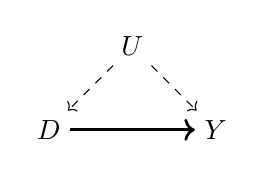
\begin{tikzpicture}[node distance=1.5cm]
	
		% nodes - for left-hand DAG %
		\node[text centered] (u) {$U$};
		\node[below right of  = u, text centered] (y) {$Y$};
		\node[below left of = u, text centered] (d) {$D$};
 
		% edges %
		\draw[->, line width=1] (d) -- (y);
		\draw[dashed, ->] (u) -- (y);
		\draw[dashed, ->] (u) -- (d);

		\end{tikzpicture}
		\end{center}
		\end{minipage}


	\end{center}

Then $D$ is endogenous due to backdoor path $D \leftarrow U \rightarrow Y$ and causal effect $D\rightarrow Y$ is not identified using the backdoor criterion.  

\end{frame}	


\begin{frame}{Instruments}
	
	
	\begin{center}
	\begin{minipage}{.5\textwidth}
	
	\begin{center}
	
	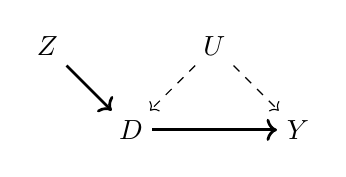
\begin{tikzpicture}[node distance=1.5cm]
	
		% nodes - for left-hand DAG %
		\node[text centered] (u) {$U$};
		\node[below right of  = u, text centered] (y) {$Y$};
		\node[below left of = u, text centered] (d) {$D$};
		\node[above left of = d, text centered] (z) {$Z$};
 
		% edges %
		\draw[->, line width=1] (d) -- (y);
		\draw[->, line width=1] (z) -- (d);
		\draw[dashed, ->] (u) -- (y);
		\draw[dashed, ->] (u) -- (d);

		\end{tikzpicture}
		\end{center}
		\end{minipage}


	\end{center}

	Notice how the path from $Z\rightarrow D\leftarrow U \rightarrow Y$ is blocked by a collider.  

\end{frame}	

